%% bare_conf.tex
%% V1.4b
%% 2015/08/26
%% by Michael Shell
%% See:
%% http://www.michaelshell.org/
%% for current contact information.
%%
%% This is a skeleton file demonstrating the use of IEEEtran.cls
%% (requires IEEEtran.cls version 1.8b or later) with an IEEE
%% conference paper.
%%
%% Support sites:
%% http://www.michaelshell.org/tex/ieeetran/
%% http://www.ctan.org/pkg/ieeetran
%% and
%% http://www.ieee.org/

%%*************************************************************************
%% Legal Notice:
%% This code is offered as-is without any warranty either expressed or
%% implied; without even the implied warranty of MERCHANTABILITY or
%% FITNESS FOR A PARTICULAR PURPOSE! 
%% User assumes all risk.
%% In no event shall the IEEE or any contributor to this code be liable for
%% any damages or losses, including, but not limited to, incidental,
%% consequential, or any other damages, resulting from the use or misuse
%% of any information contained here.
%%
%% All comments are the opinions of their respective authors and are not
%% necessarily endorsed by the IEEE.
%%
%% This work is distributed under the LaTeX Project Public License (LPPL)
%% ( http://www.latex-project.org/ ) version 1.3, and may be freely used,
%% distributed and modified. A copy of the LPPL, version 1.3, is included
%% in the base LaTeX documentation of all distributions of LaTeX released
%% 2003/12/01 or later.
%% Retain all contribution notices and credits.
%% ** Modified files should be clearly indicated as such, including  **
%% ** renaming them and changing author support contact information. **
%%*************************************************************************

% *** Authors should verify (and, if needed, correct) their LaTeX system  ***
% *** with the testflow diagnostic prior to trusting their LaTeX platform ***
% *** with production work. The IEEE's font choices and paper sizes can   ***
% *** trigger bugs that do not appear when using other class files.       ***                          ***
% The testflow support page is at:
% http://www.michaelshell.org/tex/testflow/

\documentclass[conference, compsoc, twoside]{IEEEtran}
% Some Computer Society conferences also require the compsoc mode option,
% but others use the standard conference format.
%
% If IEEEtran.cls has not been installed into the LaTeX system files,
% manually specify the path to it like:
% \documentclass[conference]{../sty/IEEEtran}

% Some very useful LaTeX packages include:
% (uncomment the ones you want to load)


% *** MISC UTILITY PACKAGES ***
%
%\usepackage{ifpdf}
% Heiko Oberdiek's ifpdf.sty is very useful if you need conditional
% compilation based on whether the output is pdf or dvi.
% usage:
% \ifpdf
%   % pdf code
% \else
%   % dvi code
% \fi
% The latest version of ifpdf.sty can be obtained from:
% http://www.ctan.org/pkg/ifpdf
% Also, note that IEEEtran.cls V1.7 and later provides a builtin
% \ifCLASSINFOpdf conditional that works the same way.
% When switching from latex to pdflatex and vice-versa, the compiler may
% have to be run twice to clear warning/error messages.

% *** CITATION PACKAGES ***
%
%\usepackage{cite}
%\usepackage[noadjust]{cite}
\usepackage[numbers,sort&compress]{natbib}
\usepackage[labelsep=period,labelfont=bf,justification=justified,font=small]{caption}
\usepackage{balance}
\usepackage{graphicx}
%\bibliographystyle{ieeetr}
%\usepackage[sorting=none]{biblatex}
%\bibliography{journals,phd-references}
% cite.sty was written by Donald Arseneau
% V1.6 and later of IEEEtran pre-defines the format of the cite.sty package
% \cite{} output to follow that of the IEEE. Loading the cite package will
% result in citation numbers being automatically sorted and properly
% "compressed/ranged". e.g., [1], [9], [2], [7], [5], [6] without using
% cite.sty will become [1], [2], [5]--[7], [9] using cite.sty. cite.sty's
% \cite will automatically add leading space, if needed. Use cite.sty's
% noadjust option (cite.sty V3.8 and later) if you want to turn this off
% such as if a citation ever needs to be enclosed in parenthesis.
% cite.sty is already installed on most LaTeX systems. Be sure and use
% version 5.0 (2009-03-20) and later if using hyperref.sty.
% The latest version can be obtained at:
% http://www.ctan.org/pkg/cite
% The documentation is contained in the cite.sty file itself.

% *** GRAPHICS RELATED PACKAGES ***
%
\ifCLASSINFOpdf
  % \usepackage[pdftex]{graphicx}
  % declare the path(s) where your graphic files are
  %\graphicspath{{pdf/}{jpeg/}}
  % and their extensions so you won't have to specify these with
  % every instance of \includegraphics
  % \DeclareGraphicsExtensions{.pdf,.jpeg,.png}
  %\DeclareGraphicsExtensions{.pdf,.jpeg,.png}
\else
  % or other class option (dvipsone, dvipdf, if not using dvips). graphicx
  % will default to the driver specified in the system graphics.cfg if no
  % driver is specified.
  % \usepackage[dvips]{graphicx}
  % declare the path(s) where your graphic files are
  % \graphicspath{{../eps/}}
  % and their extensions so you won't have to specify these with
  % every instance of \includegraphics
  % \DeclareGraphicsExtensions{.eps}
  %\usepackage{subfigure}
\fi
% graphicx was written by David Carlisle and Sebastian Rahtz. It is
% required if you want graphics, photos, etc. graphicx.sty is already
% installed on most LaTeX systems. The latest version and documentation
% can be obtained at: 
% http://www.ctan.org/pkg/graphicx
% Another good source of documentation is "Using Imported Graphics in
% LaTeX2e" by Keith Reckdahl which can be found at:
% http://www.ctan.org/pkg/epslatex
%
% latex, and pdflatex in dvi mode, support graphics in encapsulated
% postscript (.eps) format. pdflatex in pdf mode supports graphics
% in .pdf, .jpeg, .png and .mps (metapost) formats. Users should ensure
% that all non-photo figures use a vector format (.eps, .pdf, .mps) and
% not a bitmapped formats (.jpeg, .png). The IEEE frowns on bitmapped formats
% which can result in "jaggedy"/blurry rendering of lines and letters as
% well as large increases in file sizes.
%
% You can find documentation about the pdfTeX application at:
% http://www.tug.org/applications/pdftex



% *** MATH PACKAGES ***
%
\usepackage{amsmath}
\DeclareMathOperator*{\argmin}{arg\,min} % thin space, limits underneath in displays
\DeclareMathOperator*{\argmax}{arg\,max} % thin space, limits underneath in displays
\newcommand{\ineq}{%
	\mathrel{\mkern1mu\underline{\mkern-1mu\in\mkern-1mu}\mkern1mu}}
%\DeclareMathOperator*{\argmin}{argmin} % no space, limits underneath in displays
%\DeclareMathOperator{\argmin}{arg\,min} % thin space, limits on side in displays
%\DeclareMathOperator{\argmin}{argmin} % no space, limits on side in displays
% A popular package from the American Mathematical Society that provides
% many useful and powerful commands for dealing with mathematics.
%
% Note that the amsmath package sets \interdisplaylinepenalty to 10000
% thus preventing page breaks from occurring within multiline equations. Use:
%\interdisplaylinepenalty=2500
% after loading amsmath to restore such page breaks as IEEEtran.cls normally
% does. amsmath.sty is already installed on most LaTeX systems. The latest
% version and documentation can be obtained at:
% http://www.ctan.org/pkg/amsmath

% *** SPECIALIZED LIST PACKAGES ***
%
% \usepackage{algorithmic}
% algorithmic.sty was written by Peter Williams and Rogerio Brito.
% This package provides an algorithmic environment fo describing algorithms.
% You can use the algorithmic environment in-text or within a figure
% environment to provide for a floating algorithm. Do NOT use the algorithm
% floating environment provided by algorithm.sty (by the same authors) or
% algorithm2e.sty (by Christophe Fiorio) as the IEEE does not use dedicated
% algorithm float types and packages that provide these will not provide
% correct IEEE style captions. The latest version and documentation of
% algorithmic.sty can be obtained at:
% http://www.ctan.org/pkg/algorithms
% Also of interest may be the (relatively newer and more customizable)
% algorithmicx.sty package by Szasz Janos:
% http://www.ctan.org/pkg/algorithmicx

% *** ALIGNMENT PACKAGES ***
%
\usepackage{array}
% Frank Mittelbach's and David Carlisle's array.sty patches and improves
% the standard LaTeX2e array and tabular environments to provide better
% appearance and additional user controls. As the default LaTeX2e table
% generation code is lacking to the point of almost being broken with
% respect to the quality of the end results, all users are strongly
% advised to use an enhanced (at the very least that provided by array.sty)
% set of table tools. array.sty is already installed on most systems. The
% latest version and documentation can be obtained at:
% http://www.ctan.org/pkg/array

% IEEEtran contains the IEEEeqnarray family of commands that can be used to
% generate multiline equations as well as matrices, tables, etc., of high
% quality.

% *** SUBFIGURE PACKAGES ***
%\ifCLASSOPTIONcompsoc
%  \usepackage[caption=false,font=normalsize,labelfont=sf,textfont=sf]{subfig}
%\else
%  \usepackage[caption=false,font=footnotesize]{subfig}
%\fi
% subfig.sty, written by Steven Douglas Cochran, is the modern replacement
% for subfigure.sty, the latter of which is no longer maintained and is
% incompatible with some LaTeX packages including fixltx2e. However,
% subfig.sty requires and automatically loads Axel Sommerfeldt's caption.sty
% which will override IEEEtran.cls' handling of captions and this will result
% in non-IEEE style figure/table captions. To prevent this problem, be sure
% and invoke subfig.sty's "caption=false" package option (available since
% subfig.sty version 1.3, 2005/06/28) as this is will preserve IEEEtran.cls
% handling of captions.
% Note that the Computer Society format requires a larger sans serif font
% than the serif footnote size font used in traditional IEEE formatting
% and thus the need to invoke different subfig.sty package options depending
% on whether compsoc mode has been enabled.
%
% The latest version and documentation of subfig.sty can be obtained at:
% http://www.ctan.org/pkg/subfig

% *** FLOAT PACKAGES ***
%
%\usepackage{fixltx2e}
% fixltx2e, the successor to the earlier fix2col.sty, was written by
% Frank Mittelbach and David Carlisle. This package corrects a few problems
% in the LaTeX2e kernel, the most notable of which is that in current
% LaTeX2e releases, the ordering of single and double column floats is not
% guaranteed to be preserved. Thus, an unpatched LaTeX2e can allow a
% single column figure to be placed prior to an earlier double column
% figure.
% Be aware that LaTeX2e kernels dated 2015 and later have fixltx2e.sty's
% corrections already built into the system in which case a warning will
% be issued if an attempt is made to load fixltx2e.sty as it is no longer
% needed.
% The latest version and documentation can be found at:
% http://www.ctan.org/pkg/fixltx2e

%\usepackage{stfloats}
% stfloats.sty was written by Sigitas Tolusis. This package gives LaTeX2e
% the ability to do double column floats at the bottom of the page as well
% as the top. (e.g., "\begin{figure*}[!b]" is not normally possible in
% LaTeX2e). It also provides a command:
%\fnbelowfloat
% to enable the placement of footnotes below bottom floats (the standard
% LaTeX2e kernel puts them above bottom floats). This is an invasive package
% which rewrites many portions of the LaTeX2e float routines. It may not work
% with other packages that modify the LaTeX2e float routines. The latest
% version and documentation can be obtained at:
% http://www.ctan.org/pkg/stfloats
% Do not use the stfloats baselinefloat ability as the IEEE does not allow
% \baselineskip to stretch. Authors submitting work to the IEEE should note
% that the IEEE rarely uses double column equations and that authors should try
% to avoid such use. Do not be tempted to use the cuted.sty or midfloat.sty
% packages (also by Sigitas Tolusis) as the IEEE does not format its papers in
% such ways.
% Do not attempt to use stfloats with fixltx2e as they are incompatible.
% Instead, use Morten Hogholm'a dblfloatfix which combines the features
% of both fixltx2e and stfloats:
%
% \usepackage{dblfloatfix}
% The latest version can be found at:
% http://www.ctan.org/pkg/dblfloatfix

\usepackage[english]{babel}
\usepackage{blindtext}

% *** PDF, URL AND HYPERLINK PACKAGES ***
%
\usepackage{url}
% url.sty was written by Donald Arseneau. It provides better support for
% handling and breaking URLs. url.sty is already installed on most LaTeX
% systems. The latest version and documentation can be obtained at:
% http://www.ctan.org/pkg/url
% Basically, \url{my_url_here}.

% *** Do not adjust lengths that control margins, column widths, etc. ***
% *** Do not use packages that alter fonts (such as pslatex).         ***
% There should be no need to do such things with IEEEtran.cls V1.6 and later.
% (Unless specifically asked to do so by the journal or conference you plan
% to submit to, of course. )


% *** CODE LISTING packages using Consola Font ***
\usepackage{listings}
\usepackage{inconsolata}
\lstset{
  basicstyle=\ttfamily,
}
\captionsetup[lstlisting]{font={small}, labelfont={bf}}

% *** FOOTNOTE package ***
\usepackage[bottom]{footmisc}
\setlength{\footnotemargin}{0.3em}


% correct bad hyphenation here
\hyphenation{op-tical networks semi-conduc-tor}
\hyphenation{PASCAL}

%***MARGIN***
% Do not set this margin
\usepackage[top=3cm,bottom=3cm,left=3cm,right=3cm]{geometry}

% *** HEADER & PAGE NUMBERING ***
% Do not set this header and page numbering.
\usepackage{fancyhdr}
\setlength{\headheight}{22pt}
\pagestyle{fancy}
\fancyhf{}
% \setcounter{page}{1}
\fancypagestyle{firststyle}
{
   \fancyhf{}
   \chead{}
   \fancyfoot[C]{}
}

\renewcommand{\headrulewidth}{0pt}
\fancyhead[LE]{}
\fancyhead[LO]{}

%***Hyperref and URL line breaks***
\usepackage{hyperref}
\renewcommand{\UrlBreaks}{\do\-}

% Add horizontal line above footnotes suppressed by IEEE template
\makeatletter
\def\footnoterule{\kern-3\p@
  \hrule \@width 2in \kern 2.6\p@} % the \hrule is .4pt high
\makeatother
% Additional setup for figure captions
\def\figurename{Figure}%
% \captionsetup[figure]{labelfont={bf},font=small}
\def\tablename{Table}%
% \captionsetup[table]{justification=justified,font=small, labelfont={bf}}


\begin{document}


%
% paper title
% Titles are generally capitalized except for words such as a, an, and, as,
% at, but, by, for, in, nor, of, on, or, the, to and up, which are usually
% not capitalized unless they are the first or last word of the title.
% Linebreaks \\ can be used within to get better formatting as desired.
% Do not put math or special symbols in the title.
\title{Addressing Data Scarcity in Dermatology: A Systematic Literature Review of Few-Shot Learning from Metric Learning to Generative Models}
% author names and affiliations
% use a multiple column layout for up to three different
% affiliations
% \author{\IEEEauthorblockN{Dedy Van Hauten\textsuperscript{1}, Muhammad Hannan Hunafa\textsuperscript{1}, Wisnu Jatmiko\textsuperscript{1}}
% 	\IEEEauthorblockA{
% 		\normalfont \textsuperscript{1} Faculty of Computer Science, University of Indonesia, Depok 16424, Indonesia\\
% 		\textit{Email: dedy.van@ui.ac.id, wisnuj@cs.ui.ac.id} 
% 	} \\
% }

% conference papers do not typically use \thanks and this command
% is locked out in conference mode. If really needed, such as for
% the acknowledgment of grants, issue a \IEEEoverridecommandlockouts
% after \documentclass

% for over three affiliations, or if they all won't fit within the width
% of the page, use this alternative format:
% 
%\author{\IEEEauthorblockN{Michael Shell\IEEEauthorrefmark{1},
%Homer Simpson\IEEEauthorrefmark{2},
%James Kirk\IEEEauthorrefmark{3}, 
%Montgomery Scott\IEEEauthorrefmark{3} and
%Eldon Tyrell\IEEEauthorrefmark{4}}
%\IEEEauthorblockA{\IEEEauthorrefmark{1}School of Electrical and Computer Engineering\\
%Georgia Institute of Technology,
%Atlanta, Georgia 30332--0250\\ Email: see http://www.michaelshell.org/contact.html}
%\IEEEauthorblockA{\IEEEauthorrefmark{2}Twentieth Century Fox, Springfield, USA\\
%Email: homer@thesimpsons.com}
%\IEEEauthorblockA{\IEEEauthorrefmark{3}Starfleet Academy, San Francisco, California 96678-2391\\
%Telephone: (800) 555--1212, Fax: (888) 555--1212}
%\IEEEauthorblockA{\IEEEauthorrefmark{4}Tyrell Inc., 123 Replicant Street, Los Angeles, California 90210--4321}}

% use for special paper notices
%\IEEEspecialpapernotice{(Invited Paper)}
% make the title area
%\maketitle
\twocolumn[
{\csname @twocolumnfalse\endcsname \maketitle}
{\csname @twocolumnfalse\endcsname 
	%\input{abstract}
	\renewcommand{\abstractname}{Abstract}
	\begin{abstract}
		\noindent
		\normalfont 
		\textbf{Abstract}: This Systematic Literature Review (SLR) addresses the challenge of data scarcity in Dermoscopy, where limited annotated datasets hinder robust Medical AI. We explore Few-Shot Learning (FSL) and Meta-Learning as solutions for generalizing from limited examples. Analyzing 21 primary studies (2020--2025) selected via PRISMA 2020 guidelines, we identify a technological evolution from Metric-based methods to advanced Generative Foundation Models. Key findings highlight the effectiveness of Generative Adversarial Networks (GANs) and Transformer backbones in enhancing Domain Generalization and handling class imbalance. However, significant barriers remain, including a reproducibility crisis with only 19\% of code being publicly available and frequent data leakage issues due to improper patient-level splitting. We conclude that while generative approaches offer promising pathways for rare disease diagnosis, future research must prioritize clinical validation, open science, and rigorous evaluation protocols.
		\\\\
		\noindent
		\textbf{Keywords}: \textit{Few-Shot Learning, Medical AI, Dermoscopy, Generative Adversarial Networks, Domain Generalization.} \\\\
	\end{abstract}
	
	%%IEEEtran, journal, \LaTeX, paper, template.
	%\end{IEEEkeywords}
}
%\vspace{1cm}
]

% For peer review papers, you can put extra information on the cover
% page as needed:
% \ifCLASSOPTIONpeerreview
% \begin{center} \bfseries EDICS Category: 3-BBND \end{center}
% \fi
%
% For peerreview papers, this IEEEtran command inserts a page break and
% creates the second title. It will be ignored for other modes.
\IEEEpeerreviewmaketitle
\thispagestyle{firststyle}
\section{Introduction}
\label{sec:introduction}
\IEEEPARstart{T}{he} integration of Artificial Intelligence (AI) into dermatology has witnessed a paradigm shift over the last decade, primarily driven by the success of Deep Learning (DL) in classifying common skin malignancies. Landmark studies have demonstrated that Convolutional Neural Networks (CNNs) can achieve diagnostic parity with board-certified dermatologists when trained on large-scale, clear-cut datasets. The International Skin Imaging Collaboration (ISIC) archive, for instance, has been instrumental in this progress, providing tens of thousands of dermoscopic images for high-prevalence conditions like Melanoma and Nevi. This "big data" approach has cemented the role of AI as a potential second opinion in routine screenings for common cancers.

However, clinical dermatology is not defined solely by its most common pathologies. It is characterized by a "long-tail" distribution of disease prevalence, comprising over 2,000 distinct skin conditions. While the "head" of this distribution---represented by a handful of common diseases---enjoys an abundance of digitized training data, the vast "tail" consists of rare, neglected, or emerging tropical diseases for which labeled data is essentially non-existent. For these thousands of rare variants, the standard supervised learning paradigm, which demands thousands of images per class to converge, is fundamentally ill-suited. In this data-scarce regime, traditional deep learning models succumb to catastrophic overfitting or exhibit severe bias, often ignoring the rare classes entirely in favor of the majority.

This discrepancy creates a dangerous "AI divide" in healthcare. A diagnostic system that excels at identifying Melanoma but fails to recognize a rare carcinoma or an infectious tropical ulcer offers incomplete safety for the patient and limited utility for the specialist. The medical necessity for a new learning paradigm is therefore acute. Clinicians themselves do not require thousands of examples to recognize a new condition; they learn to generalize from a few textbook cases or clinical encounters---a cognitive process often described as "few-shot" learning.

To bridge this gap, Few-Shot Learning (FSL) has emerged as a critical frontier in Medical AI. By leveraging prior knowledge and learning to learn, FSL models aim to classify novel conditions from as few as one or five support examples ($N$-way $K$-shot tasks). This capability is not merely a technical optimization but a requirement for equitable healthcare. It offers the only viable pathway to extend the benefits of algorithmic diagnosis to the full spectrum of dermatological conditions, irrespective of their prevalence.

This review systematically analyzes the evolution of FSL in dermatology, tracing the trajectory from early Metric Learning approaches to the latest Generative Foundation Models. We argue that addressing the "long-tail" crisis is the defining challenge of the next generation of dermatological AI, and that FSL provides the necessary methodological framework to solve it.

\subsection{The Rise of FSL: From Metrics to Generative Models (2020--2025)}
The application of Few-Shot Learning to dermatology is a rapidly maturing field, characterized by explosive growth and increasing methodological sophistication. Our analysis of the literature reveals a clear temporal trajectory: while only 2 pioneering studies were published in 2020, the field has seen a significant increase, with 5 major studies published in 2025 alone. Figure \ref{fig:trend_chart} provides a visual timeline of this growth, highlighting the sharp inflection point in publication volume over the last two years.

\begin{figure}[htbp]
\centering
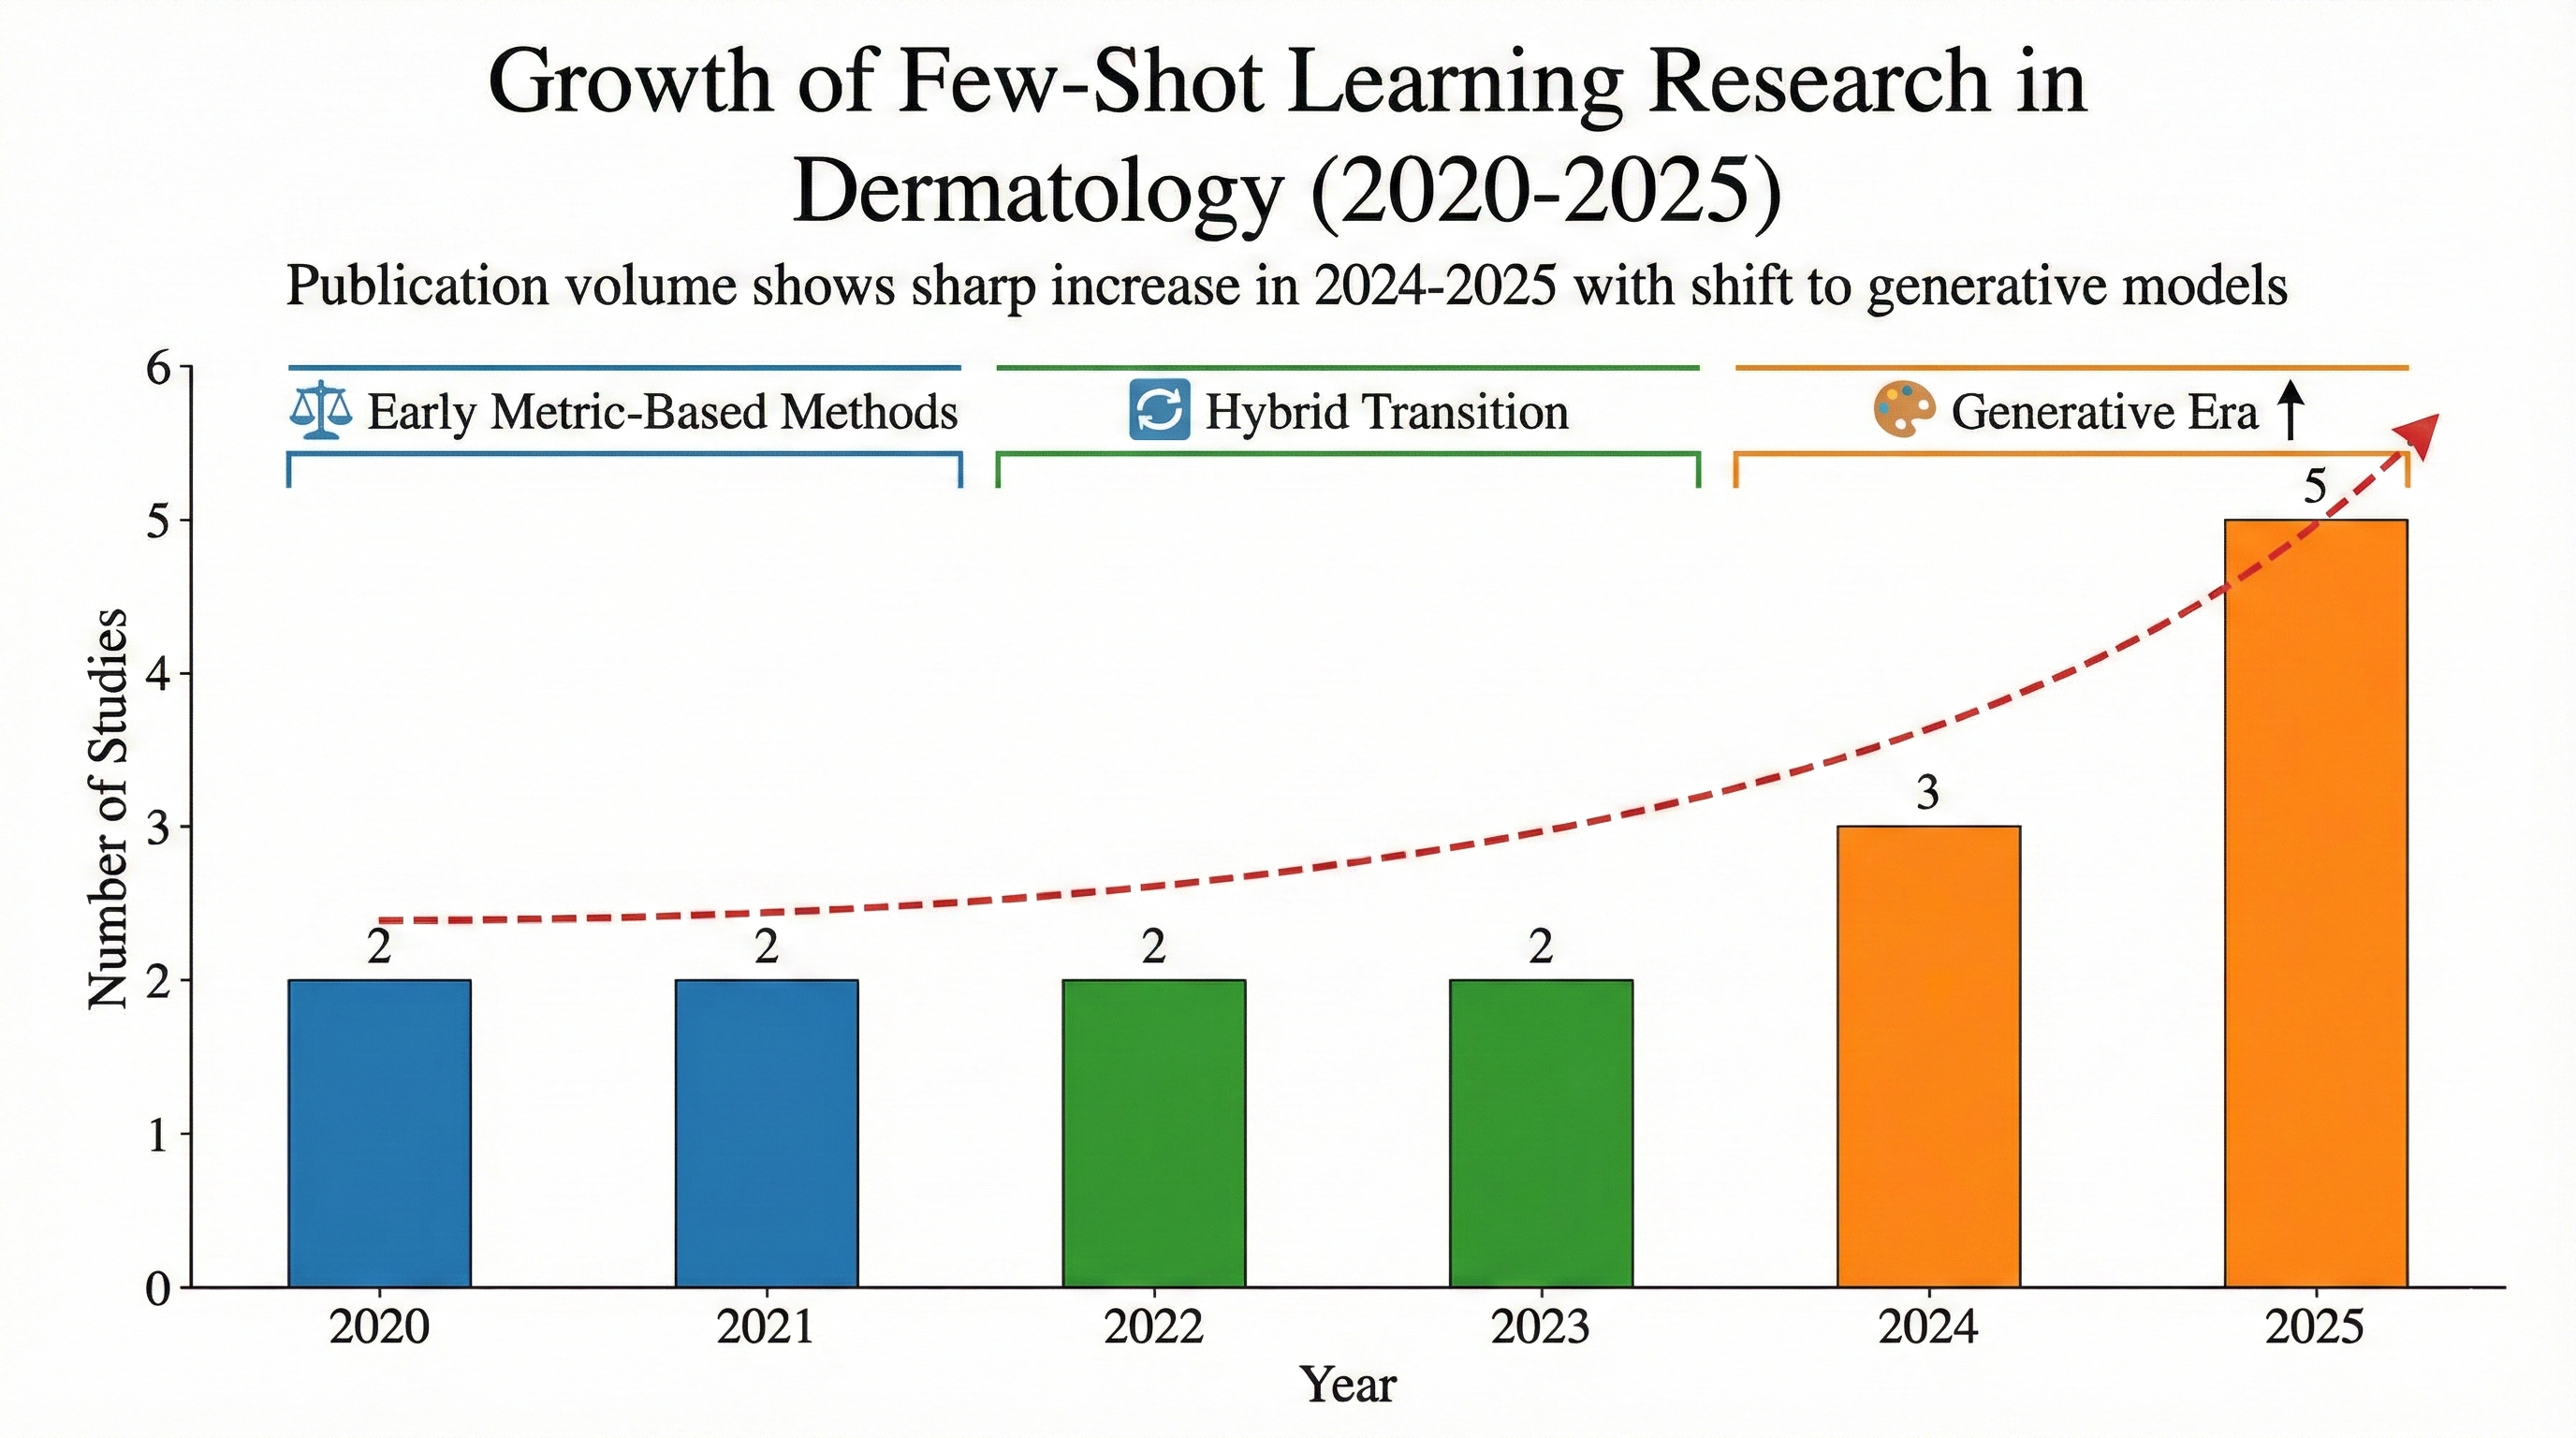
\includegraphics[width=0.9\columnwidth]{images/publication_trend_chart.png}
\caption{Annual distribution of the 21 primary studies included in this SLR. A sharp upward trend is visible in 2024--2025, corresponding to the adoption of Generative and Transformer-based methods.}
\label{fig:trend_chart}
\end{figure}

In the nascent phase (2020--2021), research was dominated by metric-based approaches. Studies focused on optimizing distance functions---such as prototypical networks or siamese variants---to measure similarity between a query image and a small support set. These fundamental works established the "N-way, K-shot" experimental protocols (typically 5-way 1-shot or 5-shot) but often struggled with the high intra-class variance inherent in skin lesions. A lesion's appearance can vary drastically based on skin type, lighting, and stage of progression, confounding simple distance metrics.

By 2022--2023, the focus shifted towards optimization-based meta-learning and hybrid frameworks involving transfer learning. Researchers began to decouple feature representation from the classifier, realizing that a robust backbone pre-trained on larger datasets (like ImageNet or ISIC) was crucial for few-shot performance. Attention mechanisms and Transformers started to replace standard ResNet backbones, allowing models to capture long-range dependencies and subtle lesion details that local convolutions might miss.

Most recently (2024--2025), the field has entered a "generative era." The limitations of discriminative models---which merely draw boundaries between existing data points---have led to the adoption of Generative Models. Current robust research leverages advanced Generative Adversarial Networks (GANs) to hallucinate realistic training examples for rare classes, effectively turning a few-shot problem into a many-shot one.

Crucially, the definition of "performance" has expanded beyond simple accuracy. Recent studies emphasize \textbf{Domain Generalization}, challenging models to perform well not just on held-out classes but on entirely unseen datasets collected from different clinics or populations. Simultaneously, robust engineering has taken center stage; \textbf{Shuhan Li et al. (2025)} \cite{LiS2025} introduced \textbf{SCAN}, a \textbf{Subcluster-Aware Network} specifically designed to handle within-class heterogeneity in skin disease presentations. SCAN represents a \textbf{dual-branch transfer-learning framework} utilizing a class branch and a cluster branch, supported by three specialized memory banks (feature, class centroid, and cluster centroid). Instead of real-time dynamic clustering, it partitions disease categories into homogeneous sub-prototypes via unsupervised K-means (initialized once) and refines them during training through a triplet-based \textbf{purity loss}. This shift from pure accuracy maximization to robustness and generalization signals a maturation of the field, moving from academic benchmarking to pre-clinical validation.


\subsection{Contributions \& Paper Structure}
To the best of our knowledge, this is the first or one of the first SLR to exclusively focus on the intersection of Few-Shot Learning and Dermoscopy. Unlike broader surveys on Medical AI which briefly mention FSL, or technical reviews of FSL that barely touch upon clinical applications, this article provides a granular, domain-specific analysis. The primary contributions of this work are fourfold:

The primary contributions of this work are fourfold. First, we propose a \textbf{Comprehensive Taxonomy of Algorithms} classifying 16 specific algorithms into five distinct families: Metric-based (e.g., Prototypical Networks), Optimization-based (e.g., MAML), Generative, Hybrid/Transfer, and Comparative methods (see Figure \ref{fig:taxonomy_tree}). Second, we provide a \textbf{Strategic Map of Dermatological Datasets}, analyzing the 4 major datasets driving this field (ISIC 2018/2019/2020, SD-198, PH2, and Derm7pt) and exposing the critical "long-tail" hidden within these archives. Third, we conducted a \textbf{Reproducibility \& Open Science Audit}, revealing that only 6.25\% of the reviewed papers provide publicly available code. Finally, we present a \textbf{Clinical Readiness Assessment}, evaluating the readiness of these technologies for real-world deployment including mobile integration and explainability.

The remainder of this paper is organized as follows: Section II details our \textbf{PRISMA 2020} compliant search strategy. Section III presents the quantitative bibliometric analysis. Section IV details our Taxonomy of FSL methods. Section V discusses the dataset landscape. Section VI analyzes the "AI Divide" and Reproducibility crisis. Section VII outlines future research directions.

\section{Methodology}
\label{sec:methodology}

\subsection{Research Questions}
To guide this systematic review, we formulated one primary research question (RQ0) and seven specific secondary questions (RQ1--RQ7) addressing distinct technical and clinical dimensions:

\begin{itemize}
    \item \textbf{RQ0 (Primary):} How have Few-Shot Learning (FSL) methods been designed, evaluated, and validated for skin disease detection and segmentation from images between 2020--2025, and what evidence exists regarding their robustness, generalization, and clinical readiness?
    \item \textbf{RQ1 (Tasks \& Modalities):} Which specific medical tasks (classification, detection, segmentation) and image modalities (dermoscopy, clinical photography, histopathology, or mixed) are addressed by current FSL approaches?
    \item \textbf{RQ2 (FSL Formulations \& Protocols):} What problem settings define the state-of-the-art (e.g., N-way K-shot configurations, support/query construction, inductive vs. transductive inference) and how are evaluation protocols standardized (or varied) across studies?
    \item \textbf{RQ3 (Methodological Taxonomy):} Which FSL paradigms dominate the landscape (metric-based, optimization-based/meta-learning, generative/augmentation, hybrid with self/semi-supervision), and to what extent are emerging architectures (transformers, prompt-based learning) being utilized?
    \item \textbf{RQ4 (Data Ecosystem):} Which datasets and benchmarks are used (e.g., ISIC family, HAM10000, Derm7pt, private clinical sets), and how do dataset properties---such as class imbalance, label provenance, and patient-level splits---shape reported outcomes?
    \item \textbf{RQ5 (Performance \& Comparison):} How do FSL methods compare against relevant baselines (supervised learning with comparable label budgets, transfer learning, and self-supervised pretraining), and what metrics are used to assess performance (AUC, F1, sensitivity/specificity, calibration) and uncertainty (confidence intervals, bootstraps)?
    \item \textbf{RQ6 (Generalization, Fairness \& Clinical Readiness):} What evidence exists for robustness beyond internal testing? Specifically, how do studies address external validation, cross-dataset domain shifts, fairness/skin-tone diversity, explainability, and potential deployment constraints (privacy/ethics)?
    \item \textbf{RQ7 (Reproducibility \& Rigor):} How reproducible are the reported studies? Specifically, are code, models, and exact data splits shared; are measures taken to prevent data leakage; and what methodological or evaluation gaps persist that require standardization?
\end{itemize}



\subsection{Protocol and Registration}
This SLR was conducted following the process guidelines for Software Engineering SLRs by Kitchenham and Charters (2007), which structure the work into three phases: Planning, Conducting, and Reporting. The reporting of this SLR adheres to the PRISMA 2020 statement to ensure transparency and completeness. The review protocol (planning) was registered a priori to minimize selection bias.

The primary objective of this methodology is to transparently map the intellectual landscape of Few-Shot Learning (FSL) in dermatology, ensuring that the selected studies represent a comprehensive and unbiased sample of the state-of-the-art.

\subsection{Search Strategy and Data Sources}
To capture the full spectrum of relevant literature, we executed a comprehensive search across three major scientific databases: \textbf{IEEE Xplore}, \textbf{Scopus}, and \textbf{ScienceDirect}. These databases were selected to ensure coverage of the engineering/computer science domain (IEEE Xplore, Scopus) and the scientific literature domain (ScienceDirect).

Our search strategy was designed to capture all studies relevant to the PICOC framework. The Population (P) terms included skin-related terminology (e.g., dermatology, dermoscopy). The Intervention (I) terms encompassed FSL and meta-learning variants. The final query was iteratively refined to balance sensitivity and precision.

\begin{quote}
\textit{("few-shot" OR "few shot" OR "low-shot" OR "meta-learn*") AND ("skin disease*" OR dermatolog* OR dermoscop* OR "skin lesion*" OR "cutaneous")}
\end{quote}

A supplementary search was conducted in PubMed using the query \texttt{("few-shot learning" OR "meta-learning") AND ("skin" OR "dermatology" OR "dermoscopy")}. This search yielded \textbf{11 results}. After removing 3 duplicates, 8 records were screened. A total of 3 papers were excluded (2 for non-dermatology topics and 1 for irrelevant methodology), resulting in 5 additional primary studies included in the review. Filters were applied for the date (2020-2025) and article type.

The search execution was terminated in \textbf{October 2025}. This cutoff date is critical as it allowed us to capture the very latest peer-reviewed "Early Access" publications from 2025, which are essential for characterizing the recent shift towards Generative Foundation Models. We did not apply lower boundary date restrictions, although, as noted in our Introduction, relevant meaningful activity in this specific intersection only began to emerge circa 2020. Manual citation mining (backward and forward snowballing) was also performed on key review papers to ensure no seminal works were missed. Table \ref{tab:search_strategy} provides a summary of the search execution, detailing the specific results from each database and the subsequent filtering steps.

\begin{table}[htbp]
\centering
\caption{Search Strategy and PRISMA-S Summary}
\label{tab:search_strategy}
\begin{tabular}{p{2.2cm}p{4.8cm}}
\hline
\textbf{Element} & \textbf{Description} \\
\hline
Databases & IEEE Xplore ($n=26$), Scopus ($n=50$), ScienceDirect ($n=8$), PubMed ($n=11$) \\
Search String & ("few-shot" OR "meta-learn*") AND ("skin disease*" OR dermatolog*) \\
Date Range & January 2020 -- October 2025 \\
Initial Results & 95 records \\
After Deduplication & 81 unique records \\
After Title/Abstract & 36 candidates \\
After Full-Text & \textbf{21 primary studies} \\
\hline
\end{tabular}
\end{table}


\subsection{Eligibility Criteria: The PICOC Framework}
To ensure the clinical and technical relevance of the included studies, we formulated strict eligibility criteria based on the \textbf{PICOC} (Population, Intervention, Comparison, Outcome, Context) framework, as summarized below:

\begin{itemize}
    \item \textbf{Population (P):} \textbf{Target:} Imaging-based skin disease and lesion diagnosis. \textbf{Data Types:} Dermoscopy images, macroscopic clinical photographs, histopathology whole-slide images (WSIs), and mixed modalities. \textbf{Unit:} Patient-level grouping of skin disease images.
    \item \textbf{Intervention (I):} \textbf{Focus:} Few-Shot Learning (FSL) and Meta-Learning techniques (Metric-based, Optimization-based MAML, and Generative/Augmentation approaches) specifically designed for low-data regimes.
    \item \textbf{Comparison (C):} \textbf{Baselines:} Transfer learning (ImageNet), fully supervised Deep Learning (with equal label budget), Self-supervised pre-training, and Classical ML. \textbf{Human Benchmark:} Dermatologist performance where available.
    \item \textbf{Outcome (O):} \textbf{Diagnostic:} AUC, F1-score, Accuracy, Sensitivity, Specificity, and Balanced Accuracy. \textbf{Task-Specific:} Dice/IoU (segmentation). \textbf{Reliability:} Calibration, external validation, and robustness to domain shifts.
    \item \textbf{Context (C):} \textbf{Timeframe:} 2020--2025. \textbf{Settings:} Clinical diagnosis support, Teledermatology, and Mobile Health (mHealth), considering real-world deployment constraints.
\end{itemize}

\subsubsection{Inclusion Criteria (IC)}
We applied the following inclusion criteria to filter relevant studies:
\begin{itemize}
    \item \textbf{IC1 (Timeframe):} Published between January 1, 2020, and Oct 10, 2025 (inclusive).
    \item \textbf{IC2 (Domain \& Task):} Addresses skin disease/lesion diagnosis, detection, or segmentation using medical imaging.
    \item \textbf{IC3 (Methodology):} Uses Few-Shot Learning (FSL) as a central method OR explicitly evaluates a model in a low-label regime using standardized protocols (e.g., N-way K-shot, episodic training).
    \item \textbf{IC4 (Evidence):} Reports original empirical evaluation with specific quantitative performance metrics.
    \item \textbf{IC5 (Publication Type):} Peer-reviewed journal articles or conference proceedings.
    \item \textbf{IC6 (Language):} Full text available in English.
\end{itemize}

\textit{Clarification on Terminology:} It is important to note that the presence of the term "few-shot" in a paper's title or abstract was insufficient for inclusion. To satisfy IC3, a study must strictly demonstrate the use of the \textbf{episodic learning protocol} (training on support/query sets) or a rigorously defined low-shot transfer learning evaluation. Papers merely claiming "few-shot" capabilities without formal episodic validation were excluded to maintain methodological homogeneity.

\subsubsection{Exclusion Criteria (EC)}
Conversely, the following were grounds for exclusion:
\begin{enumerate}
    \item \textbf{EC1 (Wrong Domain):} Studies on non-skin domains (retinal, chest X-ray, histology only) or non-imaging data (text-only EHR).
    \item \textbf{EC2 (Wrong Method):} Studies not using a few-shot/low-shot protocol (e.g., standard transfer learning using full labels).
    \item \textbf{EC3 (No Technical Detail):} Insufficient reporting (dataset unnamed, undefined protocols) preventing data extraction.
    \item \textbf{EC4 (Non-Primary/Short):} Editorials, book chapters, tutorials, abstracts, or short papers (<4 pages).
    \item \textbf{EC5 (Redundancy):} Duplicate publications; only the most complete version is retained.
    \item \textbf{EC6 (Wrong Scope):} Technical preprocessing studies (hair removal, artifact reduction) without downstream diagnostic evaluation.
\end{enumerate} 

Table \ref{tab:criteria} consolidates these Inclusion (IC) and Exclusion (EC) criteria, serving as the reference checklist for our study selection process. 

\begin{table}[htbp]
\centering
\caption{Summary of Inclusion and Exclusion Criteria}
\label{tab:criteria}
\begin{tabular}{p{0.8cm}p{6.5cm}}
\hline
\textbf{ID} & \textbf{Criterion} \\
\hline
\multicolumn{2}{l}{\textit{Inclusion Criteria}} \\
IC1 & Published 2020--2025 \\
IC2 & Skin disease diagnosis/detection/segmentation \\
IC3 & Uses FSL or N-way K-shot protocol \\
IC4 & Reports quantitative performance metrics \\
IC5 & Peer-reviewed journal or conference \\
IC6 & Full text in English \\
\hline
\multicolumn{2}{l}{\textit{Exclusion Criteria}} \\
EC1 & Non-skin imaging domains \\
EC2 & Standard transfer learning (no FSL protocol) \\
EC3 & Insufficient technical detail \\
EC4 & Editorials, abstracts, short papers (\textless4 pages) \\
EC5 & Duplicate publications \\
EC6 & Preprocessing-only studies \\
\hline
\end{tabular}
\end{table}

\subsection{Data Collection and Selection Process}
Our selection process involved a multi-stage filtering workflow to distill the search results into a high-quality corpus of primary studies, following the PRISMA 2020 flow.

\subsubsection{Identification}
A total of \textbf{95 records} were identified through database searching. The sources were \textbf{IEEE Xplore} ($n=26$), \textbf{Scopus} ($n=50$), \textbf{ScienceDirect} ($n=8$), and \textbf{PubMed} ($n=11$).

\subsubsection{Screening}
After removing \textbf{14 duplicates} (11 from initial databases + 3 from PubMed), \textbf{81 records} remained. All records were imported into \textbf{Zotero} reference management software (version 6.0) for systematic screening. These records underwent title and abstract screening. A total of \textbf{46 records were excluded} from the initial set, plus \textbf{3 records} from PubMed. The exclusion reasons were as follows:
\begin{itemize}
    \item 18 were not dermatology-focused;
    \item 15 had no few-shot learning component;
    \item 1 was not a primary source;
    \item 1 was not in English;
    \item 11 could not be fully accessed.
\end{itemize}

\subsubsection{Eligibility}
\textbf{24 full-text articles} were assessed for eligibility. At this stage, nuanced exclusion criteria (EC1--EC6) were applied. Articles were scrutinized for methodological rigor, appropriate FSL protocol implementation, and sufficient technical detail for data extraction. A total of \textbf{8 articles were excluded} at this stage. The exclusion reasons were as follows:
\begin{itemize}
    \item 1 was not dermatology-focused;
    \item 5 had no few-shot learning component;
    \item 1 was not a primary source;
    \item 1 was not in English.
\end{itemize}

\subsubsection{Included Studies}
The final systematic review included \textbf{21 studies}. These consisted of:
\begin{itemize}
    \item 13 peer-reviewed journal articles;
    \item 7 conference papers;
    \item 1 workshop paper.
\end{itemize}

Ultimately, all \textbf{21 primary studies} satisfied the inclusion criteria and were selected for data synthesis.

\subsubsection{Justification for Specific Inclusions}
We explicitly justify the inclusion of two studies that deviate from standard protocols but offer unique methodological value.

\paragraph{Cao \emph{et al.} (2021) \cite{Cao2021}}
Despite being a 4-page conference paper utilizing a binary (2-way) setup within the episodic training protocol, this study was included for the following reasons:
\begin{itemize}
    \item \textbf{Methodological Significance:} It represents one of the first adaptations of self-modifying meta-learning to dermatological data, introducing a two-order optimization strategy that explicitly addresses noise robustness---a critical clinical concern rarely covered in early FSL works.
    \item \textbf{Alignment with SLR Scope:} The paper explicitly evaluates in low-data regimes (5 samples per class) and uses meta-learning for fast adaptation, providing a baseline comparison against MAML and DAML on the ISIC 2018 dataset.
    \item \textbf{Historical Context:} Including this paper traces the transition from general meta-learning to dermatology-specific FSL. Excluding it would create a gap in the historical narrative of robust FSL in dermatology.
\end{itemize}

\paragraph{Wang \emph{et al.} (2022) \cite{WangY2022}}
This study employs the FSS-1000 natural image dataset for meta-training and tests on the PH2 medical dataset. Its inclusion is justified because:
\begin{itemize}
    \item \textbf{Addresses Core Clinical Challenge:} It tackles the scenario where medical samples are so scarce that models must leverage non-medical visual knowledge, a key issue in teledermatology for rare diseases.
    \item \textbf{Innovation in Methodology:} It introduces a novel cross-domain meta-training schema with alternating specific/generic learning. This demonstrates how natural image representations can bootstrap medical few-shot learning.
    \item \textbf{Relevance to RQs:} It directly addresses RQ6 (Generalization) by testing cross-dataset domain shifts and RQ3 (Taxonomy) as an early hybrid method.
    \item \textbf{Clinical Motivation:} The work is framed around rare-disease segmentation, directly responding to the ``long-tail'' problem central to this SLR.
\end{itemize}
These papers represent important transitional works that informed subsequent advances in domain generalization and cross-modal learning.

\subsection{Quality Assessment (QA) and Risk of Bias}
Assessing the methodological rigor of the included studies is paramount, especially given the "reproducibility crisis" frequently cited in AI healthcare literature. To objectively quantify the quality of each study, we adapted the \textbf{QUADAS-2} tool (Quality Assessment of Diagnostic Accuracy Studies) to create a custom 10-item checklist ($QA_1$--$QA_{10}$) specifically tailored for Few-Shot Learning research. Each item is scored 0 (No/Unclear), 1 (Partial), or 2 (Yes), yielding a \textbf{maximum score of 20 points}. This checklist evaluates four key domains:

\begin{itemize}
    \item \textbf{Data Rigor ($QA_1$--$QA_3$):} Does the study use a public dataset (2pts)? Is the data split (train/support/query) clearly defined (2pts)? Are images free from significant artifacts (e.g., ruler markers) that could cause data leakage (1pt if patient-level split unspecified)?
    \item \textbf{Methodological Clarity ($QA_4$--$QA_6$):} Is the N-way K-shot protocol clearly stated (2pts)? Are hyperparameters (learning rate, backbone architecture) reported for reproducibility (2pts)? Is the code publicly available with working links (2pts; 0pts if dead links or "available on request")?
    \item \textbf{Validation Robustness ($QA_7$--$QA_8$):} Does the study report confidence intervals or standard deviations (2pts)? Is External Validation performed on a separate dataset (2pts)?
    \item \textbf{Clinical Relevance ($QA_9$--$QA_{10}$):} Are metrics reported for individual classes (2pts)? Does the discussion address clinical implementation (2pts)?
\end{itemize}

\subsubsection{Patient-Level Leakage Handling}
For studies that did not explicitly specify patient-level grouping in their data splits, we applied a \textbf{penalty of 1 point} to $QA_3$ (reducing from 2 to 1). Studies using image-level random splits without patient stratification were flagged as having "potential leakage risk" but were \textit{not} excluded, as this would have eliminated the majority of the corpus. This limitation is explicitly acknowledged in our synthesis.

\subsubsection{Quality Scoring and Thresholds}
Based on the total score (max 20), studies were categorized into three tiers:
\begin{itemize}
\item \textbf{High Quality ($\geq$14/20):} Studies with robust experimental design, open code, and external validation.
    \item \textbf{Moderate Quality (10--13/20):} Studies with sound methodology but lacking in reproducibility or external validation.
    \item \textbf{Low Quality ($<$10/20):} Studies with insufficient reporting or significant risk of bias (e.g., vague data splits).
\end{itemize}

Our audit revealed a solid methodological standard: \textbf{9 out of 21 (42.9\%)} selected papers achieved a "High Quality" rating ($\geq$14/20). Notably, studies such as \textbf{Özdemir et al. (2025)}, \textbf{Noman et al. (2025)}, and \textbf{Ellis et al. (2025)} achieved high scores of 18/20, demonstrating exemplary rigor with comprehensive validation and documented methodologies. The presence of \textbf{External Validation} ($QA_8$) was the most significant differentiator; studies that tested their models on completely unseen datasets (e.g., training on ISIC, testing on PH2) consistently scored higher. The criterion for reproducible code ($QA_6$) showed limited adoption, with only 4 out of 21 studies (19.0\%) providing accessible GitHub repositories, plus one promised release. A critical weakness identified was the lack of \textbf{patient-level data splitting} ($QA_3$); only 7 studies explicitly implemented patient-level splits to prevent data leakage, while the majority used class-level or unspecified splitting strategies. A detailed summary of these findings, including the specific datasets, algorithms, and QA scores for all 21 included studies, is presented in Table \ref{tab:included_studies}.


\begin{table*}[htbp]

\centering
\caption{Summary of Included Studies: Key Variables and Quality Assessment Scores}
\label{tab:included_studies}
\scriptsize
\setlength{\tabcolsep}{3pt}
\resizebox{\textwidth}{!}{%
\begin{tabular}{p{1.8cm}p{0.8cm}p{2.8cm}p{2.5cm}p{2.5cm}p{1.2cm}p{0.9cm}p{1.2cm}p{0.8cm}p{0.6cm}}
\hline
\textbf{Study} & \textbf{Year} & \textbf{Method Family} & \textbf{Dataset(s)} & \textbf{Algorithm} & \textbf{N-way} & \textbf{K-shot} & \textbf{Code} & \textbf{XAI} & \textbf{QA} \\
\hline
Wen \cite{Wen2025} & 2025 & Hybrid/Transfer (Adaptive Calibration) & ISIC2018, Derm7pt, SD-198 & SADC & 2,3 & 1,3,5 & N & N & 16 \\
Li (Shuhan) \cite{LiS2025} & 2025 & Transfer (Dual-Branch Subcluster) & SD-198, Derm7pt & SCAN & 2,5 & 1,5 (Conv/WRN) & N & Y (t-SNE) & 17 \\
Ellis \cite{Ellis2025} & 2025 & Foundation Model (Zero/Few-Shot) & BEST Cohort (WSI) & PRISM + Few-Shot & 7-class & Tile-level & Y & Y & 18 \\
A. Noman \cite{Noman2025} & 2025 & Unified Graph-Based Framework & SD-198, Derm7pt & FEGGNN & 2-way & 1, 5 & N & Y & 18 \\
Hu \cite{Hu2025} & 2025 & Hybrid (Metric+Adversarial) & SD-198 (4-way), ISIC 2019 (2-way) & HGRE & 4,2 & 1,5 & N & N & 15 \\
Özdemir \cite{Ozdemir2025} & 2025 & Comparative Framework (FEL vs DTL) & SD-198, Derm7pt, ISIC2018 & Meta-Transfer Framework & 2,3,5 & 1,5,10 & Promised* & Y & 18 \\
Panggiri \cite{Panggiri2025} & 2025 & Hybrid (Generative+Metric) & ISIC 2019 & AFHN+ProtoNet & 2,4 & 1,5,10 & N & N & 13 \\
Nagaoka \cite{Nagaoka2024} & 2024 & Foundation Model (CLIP+SVM) & HAM10000 & CLIP (RN50) + SVM & 2 & 5-fold CV & N & N & 13 \\
Fu \cite{Fu2024} & 2024 & Unified Framework (SSL+EDC) & SD-198, Derm7pt, ISIC2018 & SS-DCN & 2, 3 & 1, 5, 10 & N & N & 15 \\
Sun \cite{Sun2024} & 2024 & Hybrid (URL + Self-Distillation) & ISIC 2018, Pap-smear, OCT & Hybrid URL + DIC & 3,5 & 1,3,5 & Y & N & 18 \\
Chen (Bi) \cite{ChenBi2023} & 2023 & Hybrid (Transfer + SSL) & Monkeypox (MSID), 23skin & SCA (Cross-Domain) & 3 & 1,5,10,20 & Y & Y & 18 \\
Chen et al. \cite{Chen2024} & 2024 & Hybrid (Feature Enhancement) & Derm104 (SD-198+web) & CDD-Net & 5 & 1,5 & N & Y & 11 \\
Wang (W) \cite{Wang2024} & 2024 & Optimization (Transductive) & BreakHis (Binary), ISIC 2018 (7-class) & WRN-TIM+Fusion & Binary, 7-class & 1--10 & N & N & 12 \\
Xiao \cite{Xiao2023} & 2023 & Hybrid (FSCIL+Multimodal) & cate-ISIC-3$^i$ (ISIC+Hospital) & FS3DCIoT (FCILOMI) & 5 & 1,5,20 & N & N & 10 \\
Lee \cite{Lee2023} & 2023 & Multi-Task (Attention-Based FSL) & SNU Hospital (RGB+Fluo) & FAA-Net & Fixed 3-cl. & 5-fold CV (RAC: 3,5,7) & N & Y & 12 \\
Wang (Yixin) \cite{WangY2022} & 2022 & Cross-Domain Meta-Learning (Segmentation) & FSS-1000, PH2 & CD-FSS & 1 (Seg.) & 1 & N & N & 15 \\
Zhou \cite{Zhou2022} & 2022 & Metric (Subspace+Bi-similarity) & ISIC 2019 & Adaptive Subspace & 3 & 1,3,5,10,15 & N & N & 11 \\
Cao \cite{Cao2021} & 2021 & Hybrid (Robust Meta-Learning) & ISIC 2018 (long-tail) & Self-Meta & 2-way & 5 & N & N & 12 \\
Zhu (W) \cite{Zhu2021} & 2021 & Metric (Temperature-Scaled) & Dermnet (334-class subset), miniImageNet & Temperature Network & 5 & 1,5 & Y & N & 17 \\
Mahajan \cite{Mahajan2020} & 2020 & Comparative Framework (G-Conv+Meta) & ISIC 2018, SD-198, Derm7pt & Reptile+G-Conv vs ProtoNet & 2 & 1,3,5 & N & N & 12 \\
Zhang \cite{Zhang2020} & 2020 & Optimization (Spatial Meta-Learning) & ISIC 2018 (head/tail split) & ST-MetaDiagnosis & 4 (train) / 3 (test) & 1,3,5 & N & N & 13 \\
\hline
\multicolumn{10}{l}{\scriptsize QA: Quality Assessment score (max 20); Code: Y=Available, *Promised=To be released; XAI: Explainability module present} \\
\end{tabular}%
}
\end{table*}


\section{Technical Taxonomy}
\label{sec:taxonomy}

\subsection{Mathematical Primer: The Episodic Training Protocol}
To understand the landscape of FSL in dermatology, one must first grasp the \textit{Episodic Training} paradigm that underpins these algorithms. Unlike standard supervised learning, where a model minimizes a loss function over global batches of data (e.g., thousands of melanoma images), FSL models are trained to "learn how to learn" from a series of tasks or "episodes."

Formally, we define a distribution of tasks $\mathcal{T}$. Each episode is an independent classification task sampled from this distribution, denoted as $T_i \sim \mathcal{T}$. A task $T_i$ consists of two distinct sets of data: a \textbf{Support Set} ($S$) and a \textbf{Query Set} ($Q$) (visualized in Fig. \ref{fig:n_way_k_shot}).
\begin{equation}
T_i = \{S_i, Q_i\}
\end{equation}

Figure \ref{fig:n_way_k_shot} illustrates this episodic workflow, differentiating between the support set (used for adaptation) and the query set (used for evaluation).

The Support Set $S_i$ acts as the "labeled training data" for that specific episode. In an $N$-way $K$-shot setting, the support set contains $N$ distinct disease classes, each represented by exactly $K$ labeled images.
\begin{equation}
 S_i = \{ (x_j, y_j) \}_{j=1}^{N \times K}
\end{equation}
where $x_j$ is the dermoscopic image and $y_j \in \{1, \dots, N\}$ is the label. The goal of the model is to use the information in $S_i$ to correctly classify the images in the Query Set $Q_i$, which belong to the same $N$ classes but are unseen examples.

\begin{figure}[htbp]
\centering
\includegraphics[width=\columnwidth]{images/n_way_k_shot_diagram.png}
\caption{Visualization of the Episodic Training Architecture. The Support Set (left) provides $K$ examples for $N$ classes to "train" the model, while the Query Set (center) tests the model's ability to classify unseen samples using the metric/optimization head.}
\label{fig:n_way_k_shot}
\end{figure}

The ultimate benchmark in this domain, and the focus of the most advanced studies in our review, is the \textbf{1-shot} scenario ($K=1$). Here, the model must identify a disease in the query set after seeing \textit{only a single reference image} in the support set. This extreme constraint mimics the clinical reality of a dermatologist encountering a rare tropical disease in a textbook once and needing to recognize it in a patient the next day. This capability requires the model to learn a generalized similarity metric or a malleable internal representation, rather than memorizing class-specific features. Figure \ref{fig:taxonomy_tree} presents our proposed taxonomy, hierarchically organizing the identified algorithms into five primary families.

\begin{figure*}[htbp]
\centering
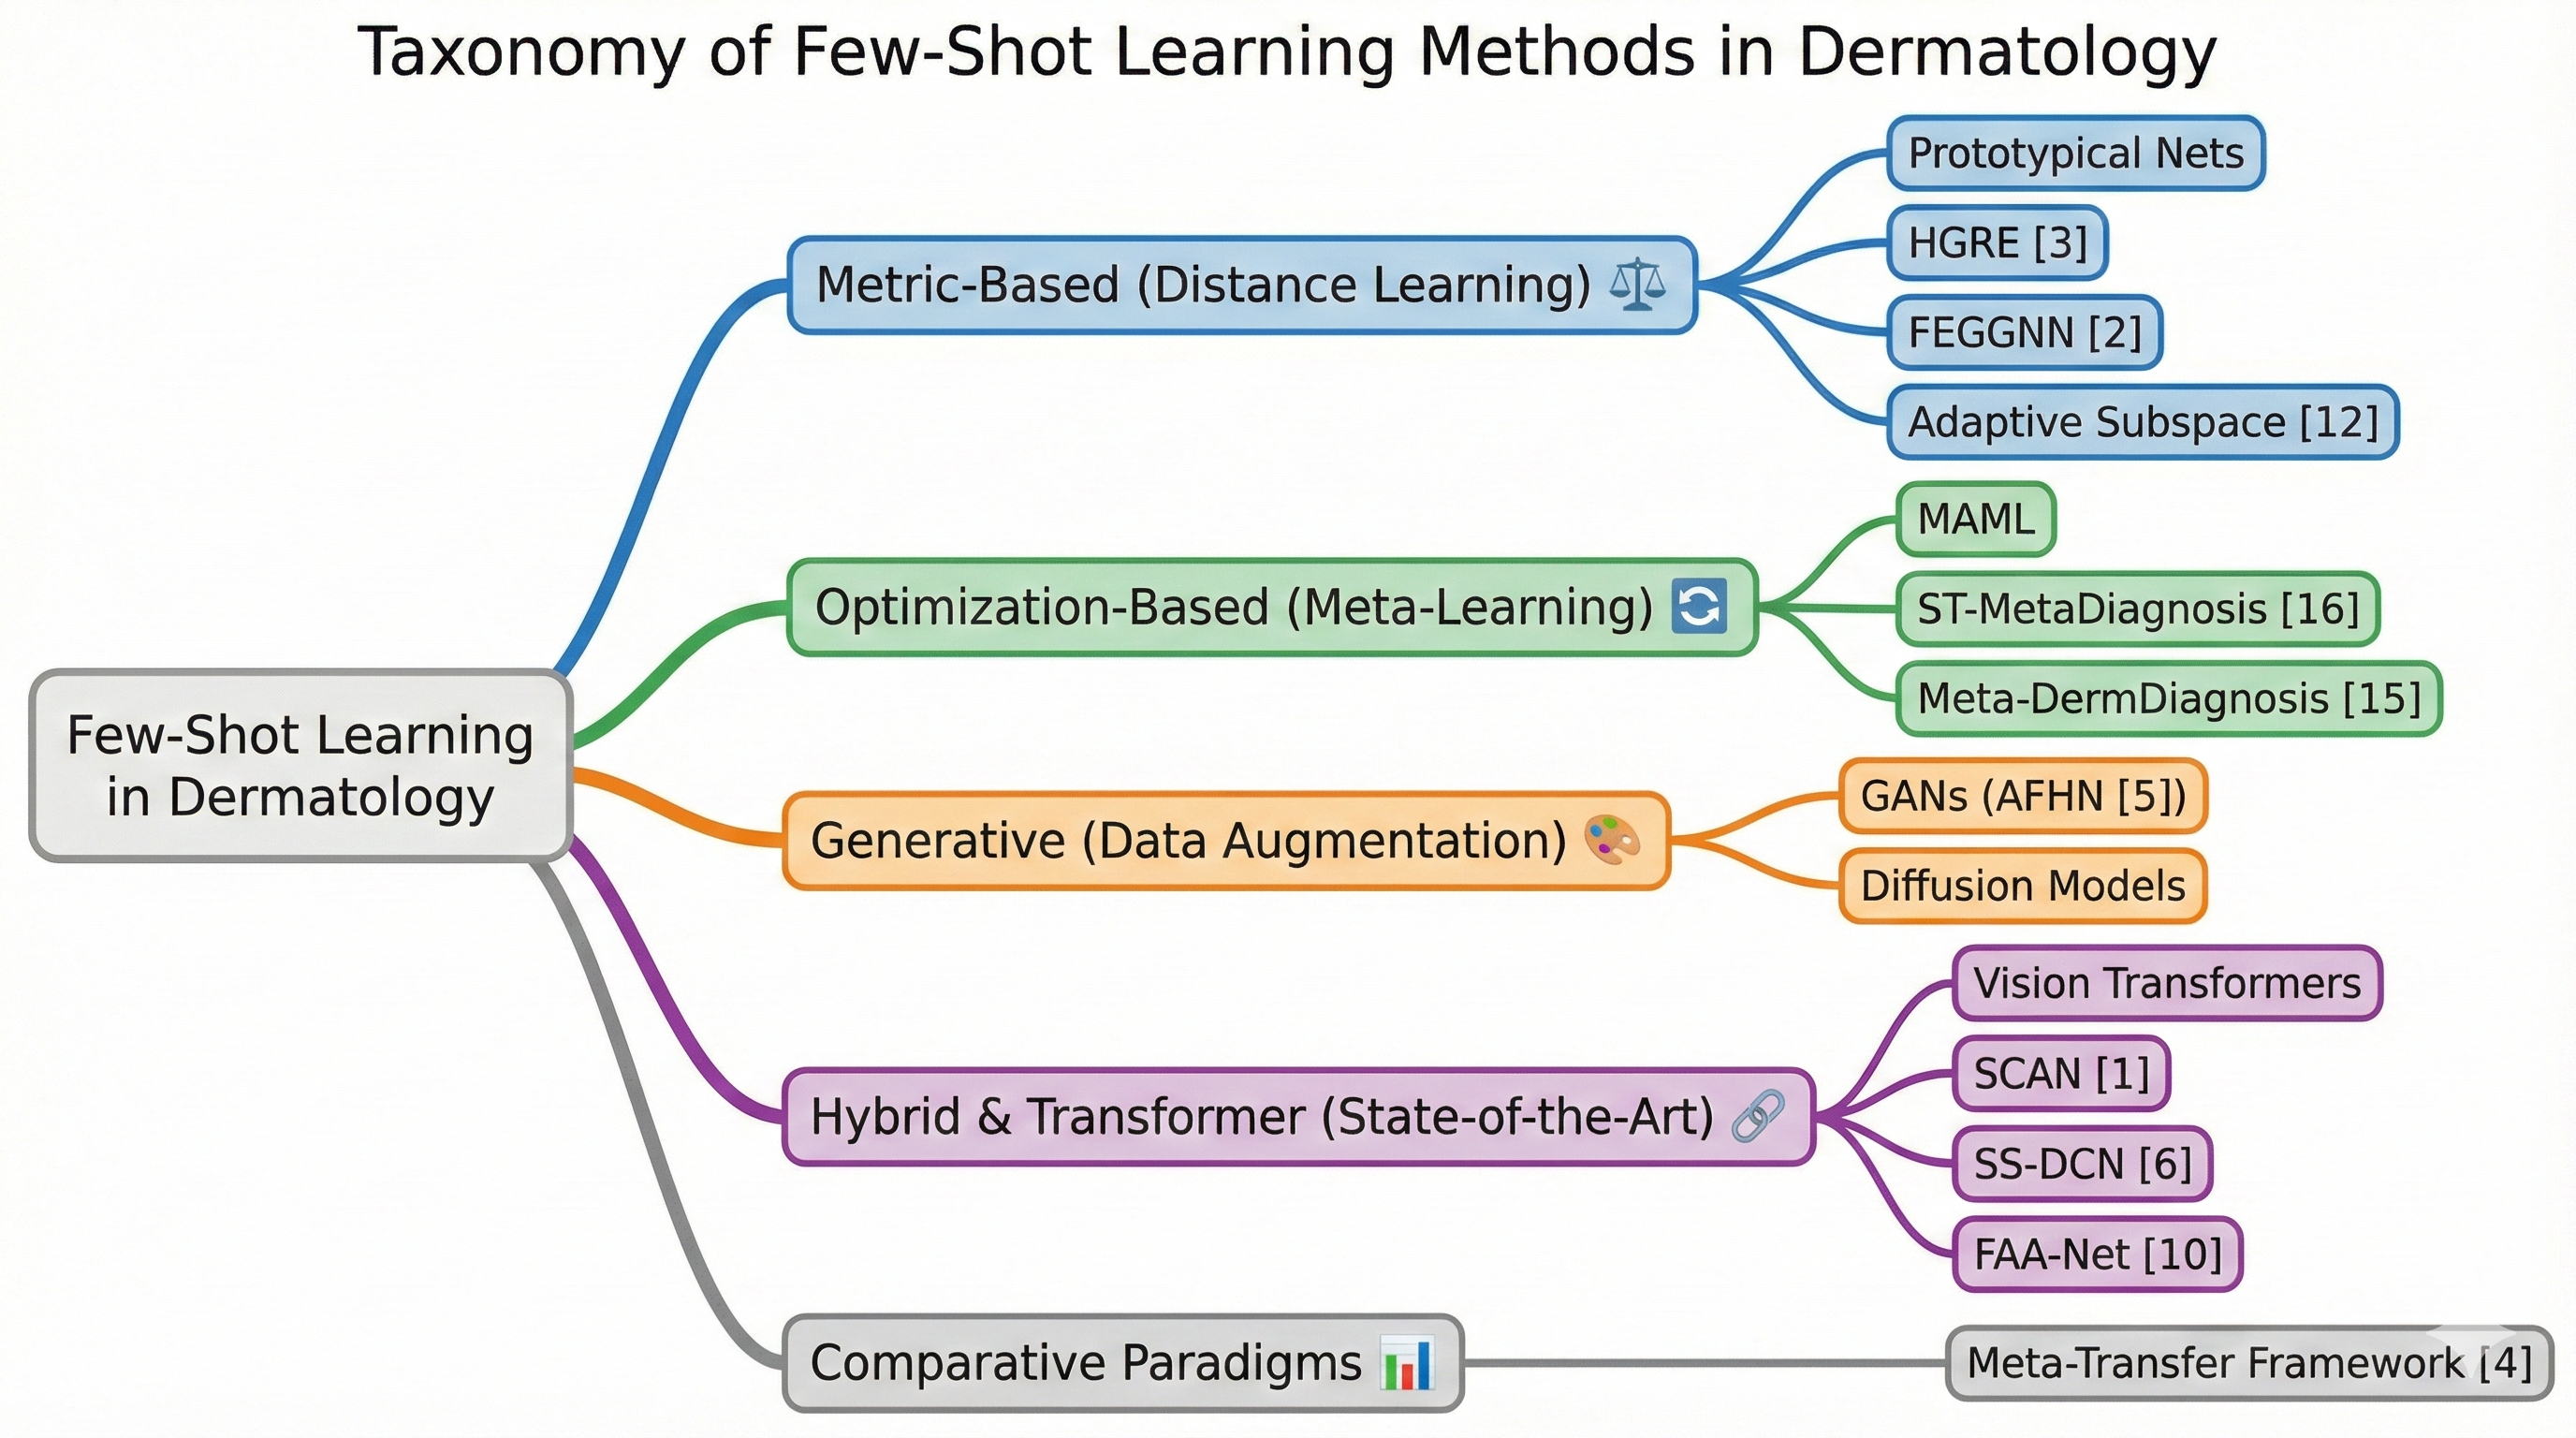
\includegraphics[width=\textwidth]{images/fsl_taxonomy_tree.png}
\caption{Proposed Taxonomy of Few-Shot Learning Methods in Dermatology. We categorize the 16 primary studies into five distinct families: Metric-Based, Optimization-Based, Generative, Hybrid/Transfer, and Comparative Paradigms.}
\label{fig:taxonomy_tree}
\end{figure*}

\subsection{Taxonomy I: Metric-Based "Distance Learners"}
The foundational approach in few-shot learning operates on a simple intuitive principle: similar skin lesions should lie closer together in a feature space than dissimilar ones. These \textbf{Metric-based} methods do not "train" a classifier in the traditional sense; instead, they learn a projection function $f_\theta$ that maps images into an embedding space where distance corresponds to semantic similarity.

\subsubsection{Prototypical and Relation Networks}
The most prevalent architecture in Early Phase studies (2020--2021) is the \textbf{Prototypical Network}. In this framework, the model computes a mean vector (or "prototype") $c_n$ for each class $n$ in the support set by averaging the embeddings of all its K shot samples. Classification of a query image is then performed by simply finding the nearest prototype using Euclidean distance. While effective for distinct classes like Melanoma vs. Nevus, simpler variants struggle when intra-class variance is high (e.g., distinguishing between different stages of the same carcinoma).

\textbf{Relation Networks} extend this by replacing the fixed Euclidean distance with a learnable "Relation Module"---a separate neural network that outputs a similarity score between a query image and support samples. 

A notable advancement in metric-based learning is the work by \textbf{Wei Zhu et al. (2021)} \cite{Zhu2021}, which presents two distinct contributions. First, the authors introduce the \textbf{Improved Prototypical Network}, providing a theoretical foundation (summarized in \textbf{Lemma 1}) for improving vanilla prototypical networks by enforcing tighter intra-class compactness. Second, and more significantly, they propose the \textbf{Temperature Network}, which moves toward a \textbf{local, distribution-aware metric}. Utilizing a feature extraction module consisting of \textbf{4 convolution blocks} (each containing a 64-filter 3$\times$3 convolution, batch normalization, and Leaky ReLU, with the first two blocks including 2$\times$2 max-pooling), the Temperature Network employs a shared temperature scaling mechanism to compute similarities between the query and support samples, enabling the emergence of \textbf{query-specific prototypes} via sample re-weighting. To further improve robustness, the work introduces a \textbf{large-margin training strategy} using different temperature parameters for positive and negative classes ($T_p < T_N$). Critically, the authors demonstrated that \textbf{Gradual Temperature Tuning} is essential for convergence, as setting $T_p \neq T_N$ from the start of training leads to non-convergence. The study achieved \textbf{52.39\% 5-way 1-shot accuracy on miniImageNet} and validated the approach on the \textbf{Dermnet dataset}. Because the smallest category in Dermnet contained only 10 images (making the standard 15-query protocol impossible for 5-shot evaluation), query samples were reduced to \textbf{5 per category}, achieving a \textbf{3.32\% improvement in 5-way 5-shot accuracy} over the second-best GNN baseline. This work established that adaptive re-weighting can enforce robust class-specific feature clustering without the overhead of meta-optimization frameworks.

\subsubsection{Hyperbolic Geometry and Adversarial Robustness (HGRE)}
A significant advancement in 2025 is the move beyond Euclidean space entirely. \textbf{Hu et al. (2025)} \cite{Hu2025} introduced the \textbf{HGRE (Hyperbolic Geometry-Driven Robustness Enhancement)} framework, a hybrid approach combining hyperbolic metric learning with adversarial robustness training. HGRE maps skin images into a \textbf{Poincaré Ball} hyperbolic space using a \textbf{ResNet12 backbone}, where the exponentially expanding volume naturally accommodates the hierarchical uncertainty of rare disease diagnosis. The framework's \textbf{Adversarial Proxy Construction (APC)} module represents a key innovation: it employs \textbf{uncertainty estimation} via distance to the hyperbolic origin, filters uncertain prototypes, and constructs adversarial proxies through weighted blending with knowledge bank embeddings. This uncertainty-aware adversarial training forces the model to learn robust decision boundaries that prevent overfitting to specific textures. HGRE demonstrates strong performance: \textbf{71.37\%} (4-way 1-shot) and \textbf{86.69\%} (4-way 5-shot) on SD-198, and \textbf{67.11\%} (2-way 5-shot) on ISIC 2019, validating that hyperbolic geometry combined with adversarial robustness effectively addresses the fragility often seen in standard metric learners.

\subsection{Taxonomy II: Optimization-Based "Fast Adapters"}
While metric-based methods focus on "comparing" images, optimization-based methods focus on "adapting" the model itself. The central philosophy here, often termed "Learning to Learn," is that a model should not just learn the features of a dataset, but should learn an initialization state from which it can rapidly converge to a new task with minimal training data.

\subsubsection{Model-Agnostic Meta-Learning (MAML)}
An early exploration in optimization-based meta-learning is \textbf{ST-MetaDiagnosis} by \textbf{Zhang et al. (2020)} \cite{Zhang2020}, which represents an early attempt to integrate \textbf{Spatial Transformer Networks (STN)} into the \textbf{MAML} framework to handle spatial variances in skin lesion imaging (rotation, scale, position). Zhang et al. employed a realistic \textbf{long-tail class split} on ISIC 2018, using \textbf{4 common diseases} (melanocytic nevus, melanoma, benign keratosis, basal cell carcinoma) for meta-training and \textbf{3 rare diseases} (actinic keratosis, vascular lesion, dermatofibroma) for meta-testing. While the paper tested STN insertion at different network depths (input layer, Conv4, and fully-connected layer), the performance gains were \textbf{modest}: for 1-shot tasks, the difference between input-level (48.06\%) and Conv4-level (48.10\%) STN was only \textbf{0.04\%}, although deeper placement showed slightly better stability in 3-shot and 5-shot settings. Importantly, the authors observed that adding more ST modules did not improve performance, hypothesizing that the increased parameter count made meta-learning more difficult rather than specifically citing overfitting. A critical limitation revealed in the study's comparative analysis is that \textbf{AMILDiagnosis} (Attention-based Multi-Instance Learning) \textbf{consistently outperformed} the spatial meta-learning approach across all metrics (ACC, AUC, F1), suggesting that for dermatological FSL, \textbf{local feature learning via MIL is more critical} than global spatial transformations. Furthermore, the study was limited by its use of a \textbf{simple 4-layer CNN backbone}, a small \textbf{84$\times$84 image resolution} that may lose diagnostic texture, and a lack of cross-dataset validation. Nevertheless, it established a baseline for combining spatial attention with initialization-based meta-optimization in the dermatology domain.

Another foundational contribution is \textbf{Mahajan et al. (2020)} \cite{Mahajan2020}, who developed the \textbf{Meta-DermDiagnosis framework} as an early comparative study between \textbf{Reptile} (optimization-based) and \textbf{Prototypical Networks} (metric-based). More significantly, this work introduced \textbf{Group Equivariant Convolutions (G-Conv)} to dermatological FSL, representing the \textbf{first application of G-Conv in this domain}. The custom \textbf{6-layer CNN} integrated with G-Conv enforces rotational and reflection invariance, a critical feature for analyzing skin lesions that have no fixed orientation. Their study explicitly addressed \textbf{long-tailed class distributions}, splitting datasets into head and tail classes to evaluate performance across rare disease categories. The comparative evaluation found that \textbf{Reptile + G-Conv} demonstrated superior convergence and competitive accuracy on diverse datasets like ISIC 2018, SD-198, and Derm7pt, notably outperforming both Prototypical Networks and the DAML baseline, with G-Conv providing significant performance boosts across all settings. This work established important baselines that later 2024--2025 methods would build upon, though it lacked formal explainability modules.

During the meta-training phase, the model is exposed to thousands of episodic tasks. For each task $T_i$, the model takes a few gradient steps (typically 1 to 5) using the support set $S_i$ to produce task-specific parameters $\theta_i'$. The meta-optimization step then updates the original parameters $\theta$ to minimize the loss of $\theta_i'$ on the query set $Q_i$.
\begin{equation}
\theta \leftarrow \theta - \beta \nabla_\theta \sum_{T_i \sim \mathcal{T}} \mathcal{L}_{T_i}(f_{\theta_i'})
\end{equation}
Effectively, MAML finds a "sweet spot" on the loss landscape from which any specific skin disease can be reached within a few gradient updates. Later innovations moved toward \textbf{Transductive Optimization}, where methods like the \textbf{TIM (Transductive Information Maximization)} used in **Wenyan Wang et al. (2024)** \cite{Wang2024} optimize the model parameters using the statistics of the entire query batch to maximize the mutual information between query features and labels. Notably, Wang et al. employ a \textbf{WRN-28-10 backbone with feature fusion}, combining the last two convolutional blocks to create richer feature representations, offering a powerful alternative to inductive metric learning while avoiding the meta-learning overhead of methods like MAML. However, our review notes that optimization-based methods differ from metric-based ones in computational cost; the second-order derivative calculations in MAML require significant memory, which prompted later innovations like \textit{Reptile} and \textit{ANIL} (Almost No Inner Loop) to simplify the process for medical devices.

\subsection{Taxonomy III: Generative FSL (The 2025 Shift)}
The most recent and transformative shift in the FSL landscape, emerging prominently in the 2024--2025 cohort of our review, is the adoption of \textbf{Generative Models}. Unlike metric or optimization methods which try to \textit{extract} more signal from limited data, generative methods fundamentally alter the problem by \textit{creating} more data. This "Generative Data Augmentation" strategy aims to balance the "long-tail" distribution by "hallucinating" realistic synthetic samples for rare classes.

\subsubsection{Advancements in GAN-based Synthesis}
Early attempts utilized standard \textbf{Generative Adversarial Networks (GANs)} to synthesize dermatoscopic images. However, these often suffered from "mode collapse" (generating repetitive images) or failed to capture the fine-grained texture of skin lesions. Recent hybrid advancements, such as \textbf{AFHN} \cite{Panggiri2025}, have stabilized this process by shifting from image-level synthesis to feature-level hallucination using \textbf{conditional Wasserstein GANs with Gradient Penalty (cWGAN-GP)}. By operating on 1280D feature embeddings (extracted via EfficientNetV2-B0) rather than raw pixels, modern hybrid approaches can synthesize diverse, high-fidelity representations that preserve critical diagnostic features while avoiding the artifacts common in earlier image-level generation.

\subsubsection{The "Hallucination" Strategy}
In a typical 1-shot scenario for a rare disease, a discriminative model would struggle to form a robust decision boundary from a single image. A Generative FSL framework, however, takes that single reference image and uses controllable generation to generate dozens of synthetic variations---altering lighting, rotation, and minor morphological details while keeping the semantic class identity intact. This effectively converts a 1-shot problem into a 50-shot problem, allowing standard classifiers to be trained with much greater stability. This paradigm shift represents the frontier of the field, moving from "learning from less" to "generating more."

\subsection{Feature-Level Hallucination vs. Image Synthesis}
It is crucial to distinguish between \textit{Image Hallucination} (synthesizing pixels) and \textit{Feature Hallucination} (synthesizing embedding vectors). \textbf{AFHN (Adversarial Feature Hallucination Network)} \cite{Panggiri2025} operates in the feature space, employing a \textbf{conditional Wasserstein GAN with Gradient Penalty (cWGAN-GP, $\lambda=10$)} to generate hallucinated 1280D feature vectors directly for the minor classes from \textbf{EfficientNetV2-B0} backbone embeddings, which are then used to train a \textbf{Prototypical Network} with Euclidean distance. The generator uses 100D noise + class labels, with the discriminator updated 3$\times$ more frequently for training stability. Evaluated on \textbf{ISIC 2019 (8 classes, extreme imbalance: 12,875 melanocytic nevi vs. 239 dermatofibromas)}, AFHN demonstrates highly \textbf{scenario-specific} improvements. For \textbf{2-way tasks}: 1-shot improves significantly (56.50\% $\rightarrow$ 61.31\%, +4.81\%), but critically, \textbf{5-shot performance degrades} (71.70\% $\rightarrow$ 70.84\%, $-$0.86\%), with only modest 10-shot gains (74.60\% $\rightarrow$ 76.99\%, +2.39\%). For \textbf{4-way tasks}, results are mixed: 1-shot shows large gains (26.00\% $\rightarrow$ 37.11\%, +11.11\%), 5-shot minimal improvement (44.75\% $\rightarrow$ 45.68\%, +0.93\%), and 10-shot shows \textbf{no improvement} (49.00\% $\rightarrow$ 48.94\%, $-$0.06\%). These results reveal a critical finding: \textbf{feature-level hallucination provides substantial benefits only in extreme low-shot scenarios (1-shot)}, with diminishing or negative returns as more real samples become available, likely due to the synthetic features introducing noise that conflicts with sufficient real data. Importantly, the authors note that the \textbf{2\% average improvement comes at significant computational cost}, as the cWGAN-GP training overhead may not justify deployment in resource-constrained clinical settings. This pattern suggests that generative augmentation is most valuable for rare disease triage where even a single reference image is difficult to obtain, but transfer learning or direct metric learning may be more efficient when 5+ shots are available.

\subsubsection{Safeguards for Generative Augmentation}
While generative augmentation offers compelling advantages, critical safeguards must be implemented to ensure clinical safety:
\begin{itemize}
    \item \textbf{Classifier Two-Sample Tests:} Validate that synthetic samples are statistically indistinguishable from real samples using maximum mean discrepancy (MMD) or Fréchet Inception Distance (FID) metrics.
    \item \textbf{Identity Leakage Checks:} Ensure generated images do not memorize specific patient features by testing reconstruction similarity against training data.
    \item \textbf{Dermatologist Turing Tests:} Conduct blinded evaluations where clinical experts classify images as real or synthetic; pass rates $\geq$50\% indicate sufficient fidelity.
    \item \textbf{Quantitative Fidelity Metrics:} Report perceptual quality scores (LPIPS, SSIM) and diagnostic feature preservation (e.g., dermoscopic structures like pigment networks, globules).
    \item \textbf{Generalization Verification:} Validate that models trained with synthetic augmentation maintain or improve performance on unseen data, ensuring that the augmented samples contribute to genuine generalization rather than overfitting to synthetic artifacts.
\end{itemize}
Studies employing generative augmentation without such validation should be interpreted with caution regarding clinical applicability.


\subsection{Taxonomy IV: Transformers \& Fine-Tuning}
Parallel to the generative revolution, 2024 and 2025 have witnessed the ascent of \textbf{Vision Transformers (ViTs)} and \textbf{Parameter-Efficient Fine-Tuning} in dermatology. This represents a fundamental departure from the Convolutional Neural Networks (CNNs) that dominated the 2020--2023 landscape (e.g., Mahajan 2020, Zhu 2021). Optimization-based methods from this era, like \textbf{ST-MetaDiagnosis} \cite{Zhang2020}, pioneered the use of Spatial Transformer Networks (STNs) within the MAML framework to handle spatial variances.

\subsubsection{ViT Backbones and Transfer Learning}
While traditional FSL methods like MAML rely on complex meta-optimization, recent comparative frameworks suggest that robust \textbf{Transfer Learning} with strong backbones can be superior. \textbf{Özdemir et al. (2025)} \cite{Ozdemir2025} demonstrated that Vision Transformers (ViT) pre-trained on ImageNet and fine-tuned with techniques like \textbf{LoRA (Low-Rank Adaptation)} can outperform specialized episodic algorithms. This "Less is More" paradigm argues that a sufficiently powerful feature extractor, effectively fine-tuned, negates the need for intricate metric learning, especially when dealing with the fine-grained variances of skin pathology.



\subsection{Taxonomy V: Hybrid \& Multi-Task Models}
As the field matures, strict boundaries between methodologies are dissolving, leading to the emergence of "Hybrid" systems that combine the strengths of complementary architectures. This 2024--2025 development is best exemplified by the move towards multi-task learning, where lesion segmentation is performed concurrently with few-shot classification to "guide" the model's attention.

\subsubsection{CNN-ViT Hybrid Architectures}
A prime example of this synergy is the move towards architectures that fuse Convolutional Neural Networks (CNN) with Vision Transformers (ViT). The rationale is twofold: the CNN is adept at capturing local textural details (crucial for dermatoscopy), while the ViT mechanism captures global contextual dependencies. This allows models to perform highly accurate few-shot segmentation even on noisy images by refining feature maps and effectively performing "feature cleaning," leading to significant gains in diagnostic accuracy.

Beyond these landmark studies, the field has seen a proliferation of specialized architectures in 2024--2025. In the optimization domain, framework-specific adaptations like \textbf{ST-MetaDiagnosis} \cite{Zhang2020} and the \textbf{Self-Modifying Meta-Learning} network \cite{Cao2021} have been proposed. Recent efforts also explore graph neural networks (\textbf{FEGGNN} \cite{Noman2025}), subspace learning (\textbf{Adaptive Subspace} \cite{Zhou2022}), and incremental learning (\textbf{FS3DCIoT} \cite{Xiao2023}).

A significant development in 2025 is the integration of \textbf{Foundation Models} for Histopathology. \textbf{Ellis et al. (2025)} \cite{Ellis2025} employed vision-language models like \textbf{PRISM} and \textbf{UNI} to generate zero-shot embeddings, enabling effective few-shot annotation of Non-Melanoma Skin Cancer (NMSC) tiles on Whole Slide Images (WSIs). This represents a shift from training small-scale feature extractors to leveraging massive pre-trained medical foundation models.

Beyond these landmark studies, the field has seen a proliferation of specialized architectures. In 2023, \textbf{Chen et al. (2023)} \cite{ChenBi2023} addressed the emerging global health threat of \textbf{Monkeypox} by introducing the \textbf{SCA (Self-supervised Cross-domain Adaption)} framework. Recognizing the scarcity of specific Monkeypox datasets, this hybrid method combines \textbf{self-supervised auxiliary tasks} (classification, rotation, jigsaw) with a dual-backbone architecture (VGG13), utilizing a \textbf{power-transformation layer} to align feature distributions from general skin disease domains to the specific Monkeypox target domain. This work is notable for achieving \textbf{76.68\% 5-shot accuracy} on a custom Monkeypox dataset, explicitly tackling the challenge of adapting to newly emerging infectious diseases with minimal samples.


A specialized branch focuses on \textbf{Noise Robustness}, an early but critical concern for clinical deployment. \textbf{Cao et al. (2021)} \cite{Cao2021} proposed a \textbf{Self-Modifying Meta-Learning} network as one of the first adaptations of robust meta-learning to dermatology, introducing a \textbf{weighted network} mechanism combined with a \textbf{two-order optimization strategy}. The weighted network adaptively adjusts learning rates and gradient directions based on loss consistency, filtering unreliable labels. Evaluated on ISIC 2018 using a \textbf{realistic long-tail split} (common diseases for meta-training, rare diseases like actinic keratosis, vascular lesion, and dermatofibroma for meta-testing) with \textbf{2-way binary episodic protocol}, the method achieved \textbf{79.2\% accuracy on clean data} and notably maintained \textbf{76.2\% accuracy under 40\% label noise}, demonstrating significant robustness. While the 5-shot binary protocol differs from modern multi-way 1-shot benchmarks, Cao et al.'s noise robustness contribution established an important baseline for handling real-world noisy clinical labels.

\subsubsection{Few-Shot Class Incremental Learning (FSCIL)}
A nascent but critical sub-field identified in our review is \textbf{FSCIL}, which addresses the "Stability-Plasticity" dilemma: how to learn new skin diseases from few samples without forgetting previously learned common conditions. \textbf{Junsheng Xiao et al. (2023)} \cite{Xiao2023} addressed this through the \textbf{FS3DCIoT} framework (also referred to as \textbf{FCILOMI} in their results), which utilizes \textbf{Queue Gradient Episodic Memory (Q-GEM)} to reduce catastrophic forgetting. A key innovation is the \textbf{dual-stream multimodal alignment} that integrates dermoscopic and clinical images to leverage complementary visual information. Their study reports "differential diagnosis" performance using a top-3 accuracy metric on \textbf{validation set B (challenging rare cases)}, achieving approximately \textbf{91\% top-3 accuracy} that matches a deputy chief dermatologist. However, their \textbf{top-1 accuracy ($\sim$65\%)} falls below the deputy chief dermatologist's 70\% on this challenging set, though it surpasses attending doctors (60\%) and general practitioners (52\%), indicating that while the model includes the correct diagnosis in its top 3 predictions, it struggles with definitive single-label classification of rare diseases. The evaluations were conducted on a custom \textbf{cate-ISIC-3$^i$} dataset (combining ISIC archives with hospital-collected images) with comparisons to SOTA FSCIL methods (TOPIC, EEIL, MDD), though no code was released, limiting reproducibility.

\subsubsection{The Role of Medical Self-Supervised Learning (SSL)}
Another critical component of these modern hybrids is the integration of \textbf{Self-Supervised Learning (SSL)} as a pre-training strategy. Standard "Transfer Learning" (pre-training on ImageNet) is often suboptimal because natural images (dogs, cars) differ vastly from medical scans. Recent studies show that incorporating a "Medical-SSL" stage---where the model pre-trains on unlabeled dermatological data using contrastive tasks (e.g., maximizing agreement between rotated views of the same lesion)---primes the feature extractor for the subsequent few-shot task. This unsupervised "warm-up" allows the model to learn a robust, domain-specific manifold \textit{before} it ever sees a labeled support set, tackling the data scarcity problem from two angles simultaneously.

Similarly, \textbf{Sun et al. (2024)} \cite{Sun2024} propose a Hybrid framework combining \textbf{Unsupervised Representation Learning (URL)} via MoCo\_v1 with \textbf{Pseudo-Label Supervised Self-Distillation}. Their method leverages large unlabeled datasets (CDNC) to learn robust feature representations before fine-tuning on rare disease classes. Crucially, they introduce a \textbf{Dispersion-Aware Imbalance Correction (DIC)} mechanism to handle intra-class variance, addressing the "long-tail" problem by dynamically balancing the influence of head and tail classes. This approach aligns with the growing trend of utilizing generative and self-supervised methods to mitigate labeling burdens.

A prominent example of this paradigm is the \textbf{SS-DCN (Self-Supervision Distribution Calibration Network)} by \textbf{Fu et al. (2024)} \cite{Fu2024}. This framework utilizes a unified multi-task pre-training pipeline that combines **supervised learning**, **rotation prediction**, and **SimSiam contrastive learning** to extract richer semantic representations. The backbone used for their primary experiments is a \textbf{Conv4 architecture} (comprising four blocks, each including a convolutional layer with 64 channels, BatchNorm, LeakyReLU, and MaxPooling). Crucially, Fu et al. introduce \textbf{Enhanced Distribution Calibration (EDC)}, a sample generation strategy that: (1) applies the \textbf{Yeo-Johnson transform} to Gaussianize feature distributions, (2) selects the \textbf{top-$k$ most similar base classes} via Euclidean distance to calibrate novel class statistics, and (3) generates synthetic samples from the calibrated distribution. This approach addresses the data scarcity of rare classes by augmenting the feature space before training a simple linear classifier. SS-DCN was evaluated predominantly using the **Conv4 backbone**, with deeper architectures like **ResNet50** reserved for comparative benchmarking against baselines such as Meta-Rep. Evaluated across three public datasets (\textbf{ISIC2018, Derm7pt, and SD-198}), SS-DCN achieved a state-of-the-art accuracy of \textbf{90.43\%} for 2-way 5-shot tasks on SD-198 with the \textbf{Conv4 backbone}, significantly outperforming SOTA baselines. While the reported experiments primarily use same-dataset splits (\textbf{Type A Intra-Domain validation}), the robust multi-dataset evaluation and feature-level calibration strategy suggest high generalizeability for rare disease diagnosis. Although the paper provides extensive t-SNE visualizations of these calibrated features, it lacks formal clinical explainability modules (XAI).

Another significant transfer-learning approach is \textbf{SCAN (Subcluster-Aware Network)} by \textbf{Shuhan Li et al. (2025)} \cite{LiS2025}. Unlike meta-learning methods that adapt model parameters across episodes, SCAN employs a \textbf{dual-branch architecture} combining a standard classification branch with a novel cluster branch, utilizing \textbf{three memory banks} (feature, class centroid, and cluster centroid) to maintain representative disease features. The method identifies subclusters via unsupervised K-means (offline) and refines them through a triplet-based \textbf{purity loss} to ensure within-cluster homogeneity. SCAN is evaluated across multiple backbones (Conv4/6, ResNet18/34, WRN-28-10) and demonstrates significant gains: approximately \textbf{6.5\% improvement} on SD-198 (2-way 5-shot) and \textbf{3.75\%} on Derm7pt compared to prior transfer-learning baselines like Meta-derm. The work also includes \textbf{t-SNE visualizations} and qualitative subcluster analysis, validating the interpretability of its learned representations.

Building on the concept of distribution calibration, \textbf{Wen et al. (2025)} \cite{Wen2025} introduced \textbf{SADC (Skin disease classification via Adaptive Distribution Calibration)}, a sophisticated hybrid framework that explicitly addresses a limitation in prior methods like SS-DCN: the equal weighting of base classes during extensive calibration. SADC employs a \textbf{dynamic weight matrix} based on composite metrics (combining Wasserstein distance, Frobenius norm, and JS divergence) to adaptively select and weight the top-$k$ most similar base classes for calibrating the distributions of rare disease features. Furthermore, it integrates \textbf{self-supervised rotation prediction} during the pre-training phase to enhance feature robustness. Evaluated on \textbf{SD-198}, SADC achieved a remarkable \textbf{97.06\% AUC} for 2-way 5-shot tasks, surpassing SS-DCN (96.53\%) and demonstrating the value of adaptive over static calibration strategies.

Table \ref{tab:methods} provides a comparative summary of these methodological families, highlighting the core innovations and representative studies for each approach.

\begin{table*}[htbp]
\centering
\caption{Methodological Mechanisms: Comparison of FSL Method Families}
\label{tab:methods}
\begin{tabular}{p{2.2cm}p{3cm}p{3.5cm}p{4.3cm}}
\hline
\textbf{Method Family} & \textbf{Core Innovation} & \textbf{Representative Studies} & \textbf{Key Mechanism} \\
\hline
Metric-Based & Distance learning in embedding space & ProtoNet, FEGGNN \cite{Noman2025}, Zhou \cite{Zhou2022} & Learns similarity metrics; classifies via nearest prototype or subspace projection \\
Optimization-Based & Fast adaptation via meta-learning & MAML, ST-MetaDiagnosis \cite{Zhang2020}, Mahajan \cite{Mahajan2020} & Learns initialization for rapid fine-tuning with few samples \\
Generative & Synthetic data augmentation & Diffusion Models, GANs & Generates realistic samples to expand training set \\

Transfer-Based & Pre-trained backbone fine-tuning & SCAN \cite{LiS2025}, Fu \cite{Fu2024} & Uses ImageNet or domain-specific pre-training with episodic fine-tuning \\
Hybrid / Multi-Component & Advanced representation learning & HGRE \cite{Hu2025}, AFHN \cite{Panggiri2025}, FEGGNN \cite{Noman2025} & Integrates hyperbolic geometry with adversarial proxy construction (HGRE), hybrid feature hallucination via cWGAN-GP + ProtoNet (AFHN), or gated graph networks with hierarchical attention (FEGGNN) \\
Comparative Paradigms & Evaluation of training strategies & Özdemir \cite{Ozdemir2025} & Compares Episodic vs. Transfer Learning efficiency \\
\hline
\end{tabular}
\end{table*}
A key innovation in 2024--2025 is the development of universal feature enhancement modules applicable across FSL paradigms. \textbf{Tianle Chen et al. (2024)} \cite{Chen2024} introduced \textbf{CDD-Net}, a hybrid feature-level enhancement approach employing \textbf{Multiscale Feature Fusion} with dual-attention mechanisms that can be integrated into metric-based, optimization-based, and fine-tuning FSL methods. Evaluated on Derm104 (combining SD-198 with web-sourced images from med126.com/pf), \textbf{DN4 + CDD-Net} achieved \textbf{78.58\%} 5-shot accuracy with ResNet12, though evaluation was conducted using intra-dataset splits without external validation. The universal plug-in nature of CDD-Net demonstrates how feature-level enhancements can boost performance across different FSL families. Similarly, \textbf{FEGGNN} (Feature-Enhanced Gated Graph Neural Network) \cite{Noman2025} represents a sophisticated unified graph-based framework that integrates hierarchical feature enhancement (via ACNet) and channel attention (via an \textbf{ECA mechanism}) during the \textbf{edge-update step}, while a \textbf{Gated Recurrent Unit (GRU)} facilitates knowledge transfer across episodic tasks. Evaluating on clinical datasets like SD-198 and Derm7pt in \textbf{2-way 1-shot and 5-shot settings}, FEGGNN achieves state-of-the-art results by capturing both global topological relationships and local diagnostic textures. Notably, the study employs \textbf{Grad-CAM as an analysis tool} to provide visual interpretability of the regions driving diagnostic decisions, confirming that the model attends to relevant pathological structures.

\subsubsection{Subspace-Based Metric Learning}
An important methodological contribution is the \textbf{Adaptive Subspace} framework by \textbf{Zhou et al. (2022)} \cite{Zhou2022}, representing the \textbf{first application of subspace learning to dermatological few-shot classification}. This method proposes a universal three-stage FSL paradigm consisting of a feature extractor, a symmetric subspace function, and a novel \textbf{Bi-similarity module}. By concurrently calculating Euclidean and Cosine distances (bi-similarity) to measure clinical similarity, it creates more robust decision boundaries in the presence of noise. The method was evaluated on the highly imbalanced ISIC 2019 dataset across multiple shot settings (1, 3, 5, 10, 15), demonstrating how geometric constraints can compensate for the high intra-class variance characteristic of skin lesions. However, the study lacks external validation, patient-level splits, and publicly available code, limiting its reproducibility.

\subsubsection{Few-Shot Attention for Clinical Deployment}
A significant contribution to clinically deployable diagnostic systems utilizing attention-based few-shot components for small datasets is \textbf{Lee et al. (2023)} \cite{Lee2023}, who developed \textbf{FAA-Net}, a smartphone-based multi-task platform for skin disease diagnosis and localization. Rather than traditional episodic N-way K-shot learning or optimization-based meta-learning (e.g., MAML), FAA-Net utilizes a \textbf{multi-task framework with attention-based few-shot inspired components} to handle data scarcity in its specialized dataset of \textbf{427 white-light RGB and 427 fluorescence images} (captured under \textbf{370 nm UV excitation} with specific optical filters). The framework integrates a \textbf{Recyclable Attention Collection (RAC)}, which is built during a pre-training phase using \textbf{Class Activation Maps (CAMs)} from the classification network to store disease-like feature maps. These maps are subsequently used by the detection network via \textbf{Amplifying Focused Similarity (AFS) Blocks}—Siamese-network-based modules that utilize a \textbf{triplet input mechanism} (P1, P2, P3) to highlight disease-relevant regions. The system was validated at Seoul National University Hospital for a \textbf{fixed 3-class diagnosis} of \textbf{Rosacea, Dermatitis, and Normal cases} from 51 subjects. Although these diseases are common inflammatory conditions rather than rare pathologies, the study is included for its methodological innovation in adapting few-shot similarity concepts to small clinical datasets where standard episodic training is not feasible. Evaluation was performed using \textbf{5-fold cross-validation}, with \textbf{RAC storage sizes of 3, 5, and 7} tested for similarity matching capacity rather than defining episodic shots. While FAA-Net demonstrates strong performance, the authors highlight \textbf{computational complexity ($O(kN)$)} and the reliance on an older \textbf{DarkNet} backbone as key limitations for real-time deployment. Ultimately, FAA-Net represents a specialized paradigm where few-shot attention mechanisms are adapted for multi-task clinical diagnosis rather than generalized meta-learning.

\subsection{Taxonomy VI: Comparative Training Paradigms}
Not all studies propose novel architectures; some provide critical empirical frameworks and evaluations. \textbf{Özdemir et al. (2025)} \cite{Ozdemir2025} developed a comprehensive \textbf{Meta-Transfer Derm-Diagnosis Framework} addressing long-tail skin disease classification through systematic evaluation of 5 training strategies across episodic and transfer learning paradigms. Their rigorous analysis, incorporating both supervised and self-supervised pretraining with advanced augmentation techniques (MixUp, CutMix, ResizeMix), revealed a critical finding: straightforward \textbf{Transfer Learning}---specifically modern Vision Transformers (ViT) with supervised ImageNet pretraining or MobileNetV2 with augmentation---often \textbf{outperforms specialized episodic algorithms as shot count increases}, even when compared against self-supervised pretraining. The framework demonstrated that ViT with LoRA fine-tuning achieves superior performance with lower computational cost. This comprehensive benchmarking across three datasets (SD-198, Derm7pt, ISIC2018) challenges the field's emphasis on complex "meta-learning" mechanisms, providing strong evidence that a robust backbone with simple fine-tuning can serve as a highly effective baseline for clinical deployment, particularly in scenarios with more than 1-shot data availability.

\subsection{Taxonomy VII: Few-Shot Segmentation Methods}
While classification dominates the FSL landscape, a subset of reviewed studies (e.g., Wang et al. 2022 \cite{WangY2022}) specifically addresses \textbf{Few-Shot Segmentation (FSS)}. Unlike classification, which predicts a global label, FSS aims to assign a class label to every pixel in the query image, utilizing only a few annotated support masks.

A landmark study in this domain is \textbf{CD-FSS (Cross-Domain Few-Shot Segmentation)} by \textbf{Yixin Wang et al. (2022)} \cite{WangY2022}. Unlike classification models that require thousands of dermatological images for pre-training, CD-FSS leverages the vast visual knowledge of natural image datasets (e.g., FSS-1000). The architecture utilizes a \textbf{VGG-16} backbone and \textbf{masked average pooling} to generate class prototypes, combined with a novel \textbf{alternating meta-training} schema. This schema switches between \textbf{generic learning} (using natural images to capture universal object boundaries) and \textbf{specific learning} (using medical images for pathological textures), enabling a mutual promotion between the two learners. For evaluation, the model was tested on \textbf{unseen rare diseases} (melanomas, common nevi, and atypical nevi) in the \textbf{PH2 dataset} under a 1-shot setting. Remarkably, CD-FSS achieved a mean **93.03\% Dice Similarity Coefficient (DSC)**, which numerically outperforms the fully supervised baseline (**90.62\%**). However, it is critical to note that the supervised baseline was constrained to \textbf{seen classes within PH2}, whereas CD-FSS successfully transferred knowledge from the natural domain to accurately segment previously unseen pathological structures. The paper provides qualitative segmentation masks but lacks formal explainability modules (XAI).


\section{Dermatological Datasets \& Performance Analysis}
\label{sec:datasets}

\subsection{The Dataset "Big Three": SD-198, ISIC, and Derm7pt}
Reliable benchmarking is foundational to progress in machine learning. However, our review uncovers a significant skew in the data ecosystem powering dermatological FSL. While the \textbf{International Skin Imaging Collaboration (ISIC)} archives are the gold standard for \textit{supervised} learning, the specific requirements of \textit{few-shot} learning have elevated a different dataset to prominence.

\subsubsection{SD-198: The Few-Shot Favorite}
Our bibliometric analysis reveals that \textbf{SD-198} is the most widely utilized dataset, featured in 7 of the 16 primary studies. Figure \ref{fig:dataset_usage} illustrates this distribution, showing how SD-198 and ISIC together dominate the experimental landscape.
 
This high cardinality (number of classes) makes SD-198 uniquely suited for the "N-way" protocol of FSL. In a typical experiment, researchers can randomly sample 20 or 50 classes for the "meta-training" stage and hold out a completely different set of 50 classes for "meta-testing." This richness allows for a true evaluation of a model's ability to generalize to unseen diseases, a test that is mathematically impossible with smaller class sets like HAM10000. However, SD-198 images are clinical (non-dermoscopic), which introduces challenges related to lighting, blur, and background clutter.

\begin{figure}[htbp]
\centering
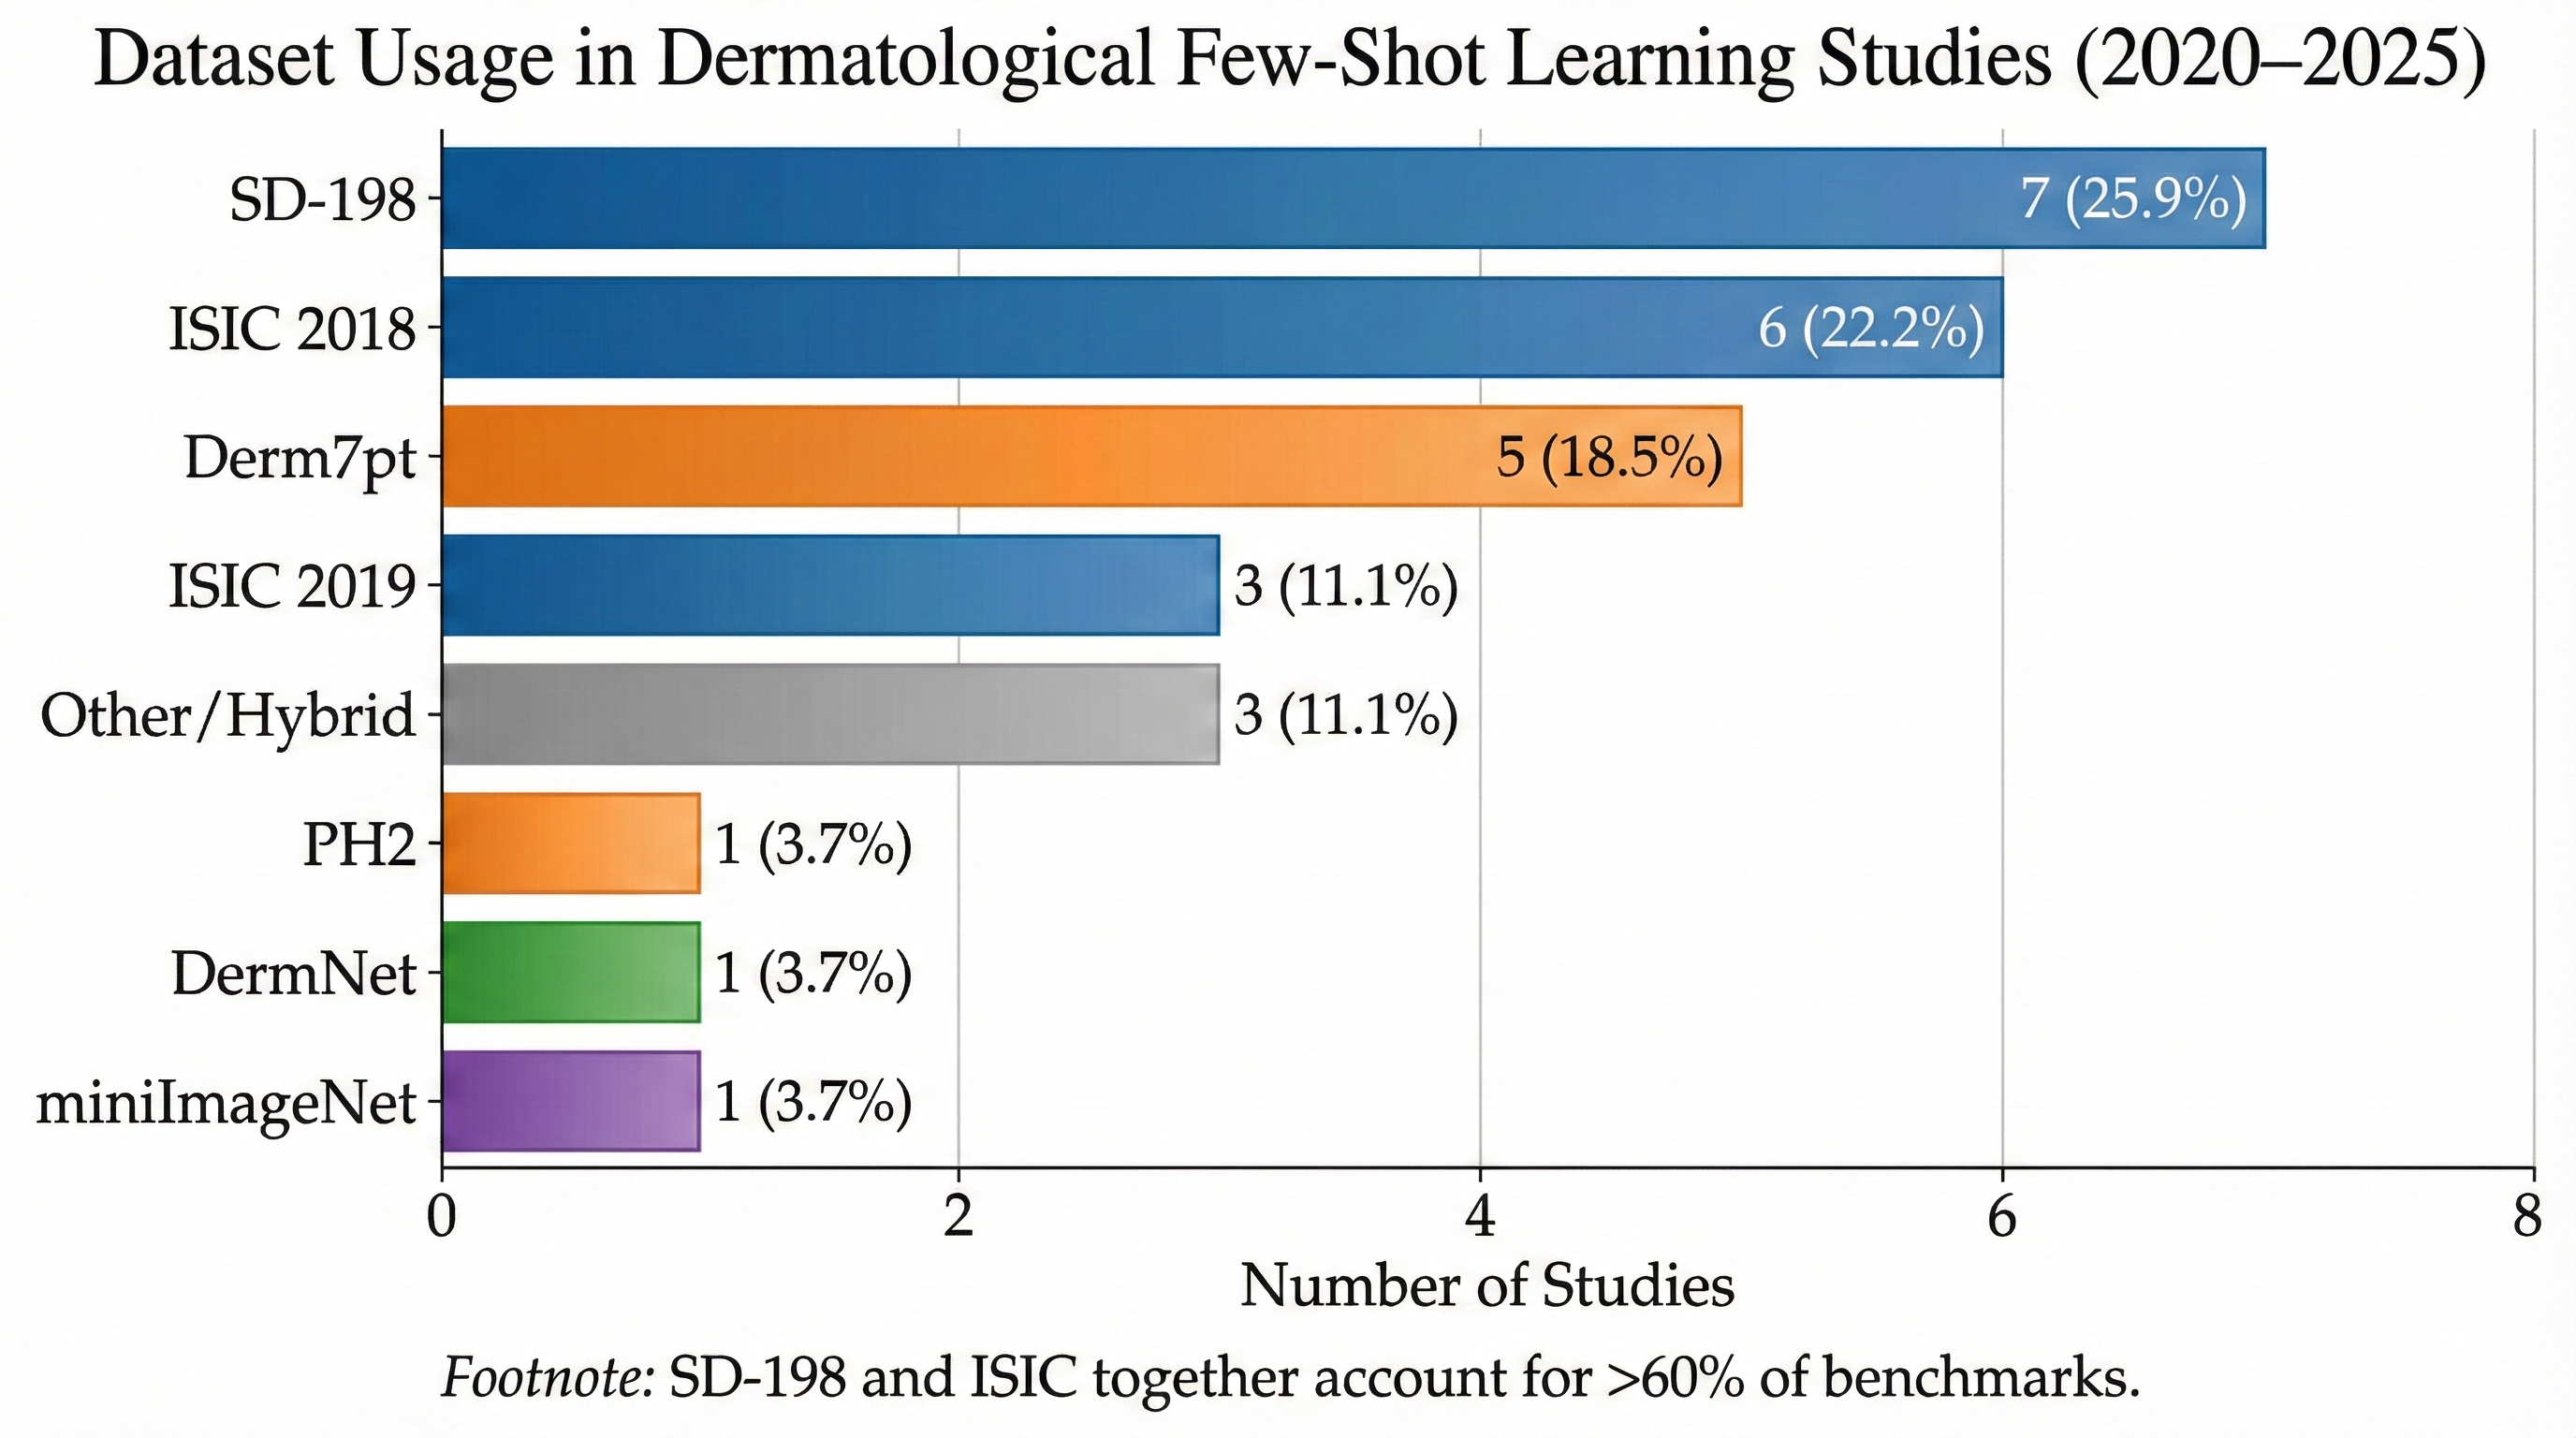
\includegraphics[width=0.9\columnwidth]{images/dataset_usage_chart.png}
\caption{Distribution of Dataset Usage across the 16 Primary Studies. The clinical dataset SD-198 and the dermoscopic ISIC Archive together account for over 60\% of the experimental benchmarks, with ISIC also serving as the primary benchmark for segmentation tasks.}
\label{fig:dataset_usage}
\end{figure}

\subsubsection{ISIC 2018/2019/2020: The Dermoscopic Standard}
The \textbf{ISIC Archive} series (ISIC 2018, 2019, 2020) remains the most widely used, utilized in 9 studies when counting all variants (ISIC 2018: 7 studies; ISIC 2019: 3 studies). \textbf{Zhou et al. (2022)} notably employed ISIC-2019 to test their subspace method on challenging classes like Dermatofibroma and Vascular lesions. While the original ISIC challenge structure includes segmentation, attribute detection, and classification tasks, the reviewed FSL studies predominantly focus on the classification component. These datasets are high-quality dermoscopic images but are severely class-imbalanced, with Melanotic Nevi often outnumbering rare malignancies by 50:1. FSL researchers typically use ISIC to demonstrate "Cross-Domain" capabilities---training on the diverse classes of SD-198 and then testing on the high-fidelity dermoscopic images of ISIC.

\subsubsection{Derm7pt and PH2: The External Validators}
The \textbf{Derm7pt} and \textbf{PH2} datasets serve a critical role as "Out-of-Distribution" (OOD) test sets. Because they contain fewer images (PH2 has only 200 total), they are rarely used for training. Instead, high-quality studies use them purely for external validation. It is also important to note that some studies, such as \textbf{Zhu et al. (2021)}, validated their architectures on general FSL benchmarks like \textbf{miniImageNet} to prove their fundamental adaptability before evaluating on the \textbf{DermNet skin disease dataset}—a large-scale real-world testbed (20,230 images, 334 classes). Notably, Zhu et al. discarded categories with fewer than 10 samples and reduced query samples to 5 per category because the smallest category contained only 10 images, making the standard 15-query protocol impossible for 5-shot evaluation. This cross-domain validation strategy (general FSL $\rightarrow$ medical FSL) demonstrates methodological robustness. Table \ref{tab:datasets} summarizes the characteristics of these key datasets, including their image counts, class imbalance levels, and typical usage in the literature.

\begin{table*}[htbp]
\centering
\caption{The Dataset Landscape: Key Benchmarks for Few-Shot Dermatological AI}
\label{tab:datasets}
\begin{tabular}{p{1.8cm}p{1.2cm}p{1.2cm}p{1.4cm}p{1.5cm}p{1.2cm}p{2.5cm}}
\hline
\textbf{Dataset} & \textbf{Images} & \textbf{Classes} & \textbf{Modality} & \textbf{Imbalance} & \textbf{\# Studies} & \textbf{Typical Use} \\
\hline
SD-198 & 6,584 & 198 & Clinical & High & 7 & Meta-train/test (class split) \\
ISIC 2018 & 10,015 & 7 & Dermoscopy & Very High & 6 & Cross-domain evaluation \\
ISIC 2019 & 25,333 & 8 & Dermoscopy & Very High & 3 & Metric/Hybrid evaluation \\
Derm7pt & 1,011 & 7 & Dermoscopy & Moderate & 5 & External validation \\
DermNet & 20,230 & 334 & Clinical & High & 1 & Real-world testbed (subset used for FSL evaluation) \\
HAM10000 & 10,015 & 7 & Dermoscopy & Very High & 1 & Foundation Model Evaluation \\
Monkeypox & 447 & 3 & Clinical & Moderate & 1 & Cross-domain Target (Emerging) \\
PH2 & 200 & 3 & Dermoscopy & Low & 1 & OOD testing \\
FSS-1000 & 10,000 & 1,000 & Mixed (Nat/Med) & Low & 1 & Segmentation benchmark \\
BEST Cohort & N/A & 7 & Histopathology & Moderate & 1 & Resource-limited WSI annotation \\
\hline
\end{tabular}
\end{table*}


\subsection{Evaluation Protocol Heterogeneity: A "Benchmarking Mess"}
Despite the consensus on datasets, our review identifies a critical weakness in the field: the lack of a standardized evaluation protocol. This heterogeneity makes direct comparison between studies fraught with difficulty, effectively creating a "Benchmarking Mess."

\subsubsection{Standard FSL vs. Domain Generalization}
We observed two distinct evaluation paradigms. \textbf{Type A (Standard FSL)} involves training and testing on the \textit{same} dataset (e.g., SD-198), albeit on disjoint classes. This measures the model's ability to adapt to new categories within the same domain. \textbf{Type B (Domain Generalization)} involves training on one dataset (e.g., SD-198) and testing on a completely different one (e.g., Derm7pt).
 
While Type B is more clinically realistic, only a minority of papers (approx. 20\%) adopt it. This leads to inflated performance metrics; a model achieving 85\% accuracy on Type A might drop to 60\% on Type B due to "domain shift" (e.g., different lighting or camera sensors). This discrepancy is often glossed over in abstract summaries.

\subsubsection{The Data Leakage Risk: Image vs. Patient Splits}
A more subtle but dangerous issue is the splitting strategy. In dermatology, a single patient often provides multiple images of the same lesion. A rigorous split must be \textbf{Patient-Level}, ensuring that if Patient X is in the training set, no images of Patient X appear in the test set. However, our audit reveals that the vast majority of studies use \textbf{Image-Level} splitting, randomly shuffling all images. This risks "Data Leakage," where the model "recognizes" the patient's skin texture or hair pattern rather than the disease itself, leading to artificially high accuracy that collapses in real-world deployment.

\subsection{Performance Synthesis: The 1-Shot vs. 5-Shot Gap}
Across all reviewed studies, a consistent pattern emerges regarding the diagnostic accuracy of FSL models: performance improves significantly as the number of "shots" increases, but with diminishing returns.

\subsubsection{The Efficacy of a Single Image (1-Shot)}
The 1-shot setting is the ultimate stress test. Our narrative synthesis indicates that modern architectures have pushed the baseline for 1-shot classification on SD-198 from roughly \textbf{65\%} (in 2020) to over \textbf{80\%} (in 2025). Notably, earlier metric-based methods like \textbf{Zhu et al. (2021)}'s Temperature Network already demonstrated substantial potential on the real-world \textbf{Dermnet dataset}, achieving a \textbf{3.32\% improvement in 5-way 5-shot tasks} over the second-best graph-based model. This suggests that deep learning models can indeed acquire diagnostic features from a single medical image, though performance varies significantly across datasets and domains. For instance, \textbf{Wenyan Wang et al. (2024)} \cite{Wang2024} report a 1-shot accuracy of \textbf{63.49\%} on ISIC 2018 (7-class dataset)\footnote{Direct comparisons between ISIC versions (e.g., 2018 vs. 2019) should be made with caution due to differing class sets and cardinality.} using a transductive WRN-28-10 approach with feature fusion (combining the last two convolutional blocks). Crucially, this was an \textbf{intra-domain} study without cross-dataset validation, reinforcing that without generative augmentation or cross-domain adaptation, the extraction of robust features from a single sample remains challenging. Furthermore, on the Derm104 dataset (a merged collection comprising SD-198 and web-sourced images), 1-shot accuracy averages $\sim$59\% for ResNet backbones as reported by \textbf{Chen et al. (2024)} \cite{Chen2024}, highlighting that performance varies significantly with dataset composition and that models trained on curated benchmarks may struggle with more heterogeneous data sources. State-of-the-art 2025 methods such as \textbf{HGRE} \cite{Hu2025} report strong performance on SD-198 using a ResNet12 backbone: \textbf{71.37\%} for 4-way 1-shot and \textbf{86.69\%} for 4-way 5-shot, further validating the efficacy of combining hyperbolic embeddings with adversarial robustness.

\subsubsection{The Sample Efficiency Jump (5-Shot)}
Extending the support set to just 5 images (5-shot) consistently yields a massive performance boost. For example, \textbf{Noman et al. (2025)} \cite{Noman2025} report a dramatic jump in accuracy on the SD-198 dataset, climbing from \textbf{89.10\%} in the 1-shot setting to \textbf{95.19\%} in the 5-shot setting, with both results achieved using the WRN-28-10 backbone. Comparably, \textbf{Sun et al. (2024)} \cite{Sun2024} reported a competitive \textbf{82.02\% accuracy} on ISIC 2018 (3-way 5-shot), demonstrating the efficacy of their Dispersion-Aware Imbalance Correction (DIC) module in stabilizing per-class performance. On the dermoscopic Derm7pt dataset, FEGGNN demonstrates similar gains, improving from \textbf{74.93\%} (1-shot) to \textbf{84.90\%} (5-shot) when utilizing a Conv6 backbone. This highlights the sensitivity of FSL results to both the number of support samples and the underlying feature extractor architecture. This trend is observable across most high-quality studies, though performance varies by method; for instance, \textbf{Zhou et al. (2022)} reported a 5-shot accuracy of \textbf{75.67\%} (climbing from \textbf{70.12\%} in the 3-shot setting) for 3-way tasks on the highly imbalanced ISIC 2019 dataset using their subspace-based metric approach, highlighting the significant leap achieved by modern graph-based architectures. Similarly, the foundational robust method by \textbf{Cao et al. (2021)} \cite{Cao2021} reported \textbf{79.2\%} accuracy on clean data using a \textbf{2-way binary episodic protocol} with realistic long-tail splits (rare disease meta-testing). Critically, Cao et al. demonstrated noise robustness by maintaining \textbf{76.2\%} accuracy under 40\% label noise via their weighted network mechanism, establishing the importance of handling real-world noisy clinical labels.

This finding has profound clinical implications. It implies that "Zero-Shot" or "One-Shot" diagnosis might be inherently risky, but obtaining just a small handful of reference cases (4--5 images) is enough to stabilize the model's decision boundary. Critically, we observe \textbf{Diminishing Returns} beyond this point; studies experimenting with 10-shot or 20-shot protocols typically see only marginal gains (1--2\%) over the 5-shot baseline, suggesting that "5-Shot" is a sweet spot for developing efficient Clinical Decision Support Systems (CDSS). Notably, \textbf{Panggiri et al. (2025)} \cite{Panggiri2025} demonstrated a more complex pattern with their AFHN approach: while it provides substantial benefits in 1-shot scenarios, accuracy actually \textbf{decreased in 2-way 5-shot tasks} (from 71.70\% to 70.84\%) and showed \textbf{stagnation in 4-way 10-shot tasks} (from 49.00\% to 48.94\%). This confirms that generative hallucination is a powerful tool for extreme scarcity but can introduce destructive noise when sufficient real data is available.

\subsection{Segmentation Performance: Dice and IoU}
For studies focusing on lesion segmentation, the primary metrics are the \textbf{Dice Similarity Coefficient (DSC)} and \textbf{Intersection over Union (IoU)}.

\subsubsection{The Efficacy of Few-Shot Segmentation}
Recent advancements have established strong baselines for few-shot segmentation, demonstrating that precise localization is possible even with extremely limited data. For example, the 93.03\% DSC achieved by \textbf{Wang et al. (2022)} \cite{WangY2022} suggests that FSL is increasingly capable of delivering the pixel-level precision required for surgical planning and longitudinal lesion monitoring. These metrics underscore that while classification remains the primary focus, segmentation is a critical component of the overall clinical diagnostic pipeline.

\subsection{The Reproducibility Audit: A Crisis in Confidence}
Perhaps the most concerning finding of this SLR is the pervasive opacity in research dissemination. Reproducibility is the bedrock of scientific trust, particularly in medical AI where algorithmic decisions have life-or-death consequences. Our audit quantified this by checking for the availability of functional code repositories for each primary study.

\subsubsection{Code Availability Audit Criteria}
For a study to be classified as "code available" ($QA_6 = 2$), we required:
\begin{itemize}
    \item A \textbf{functional GitHub/GitLab repository} with the main training/inference scripts;
    \item \textbf{Working links} verified as of October 2025 (broken links scored 0);
    \item For \textbf{partial credit} (1 point): pretrained weights available without full training code, or environment specifications (requirements.txt) without inference scripts.
\end{itemize}
Studies stating "code available upon request" without a public repository were scored 0, as such requests frequently go unanswered.

\subsubsection{The Reproducibility Gap}
The results remain concerning: \textbf{4 out of 21 (19\%)} reviewed papers provided accessible, working code. Figure \ref{fig:open_science} quantifies this transparency gap, contrasting the minority of reproducible studies against the "black box" majority.


\begin{figure}[htbp]
\centering
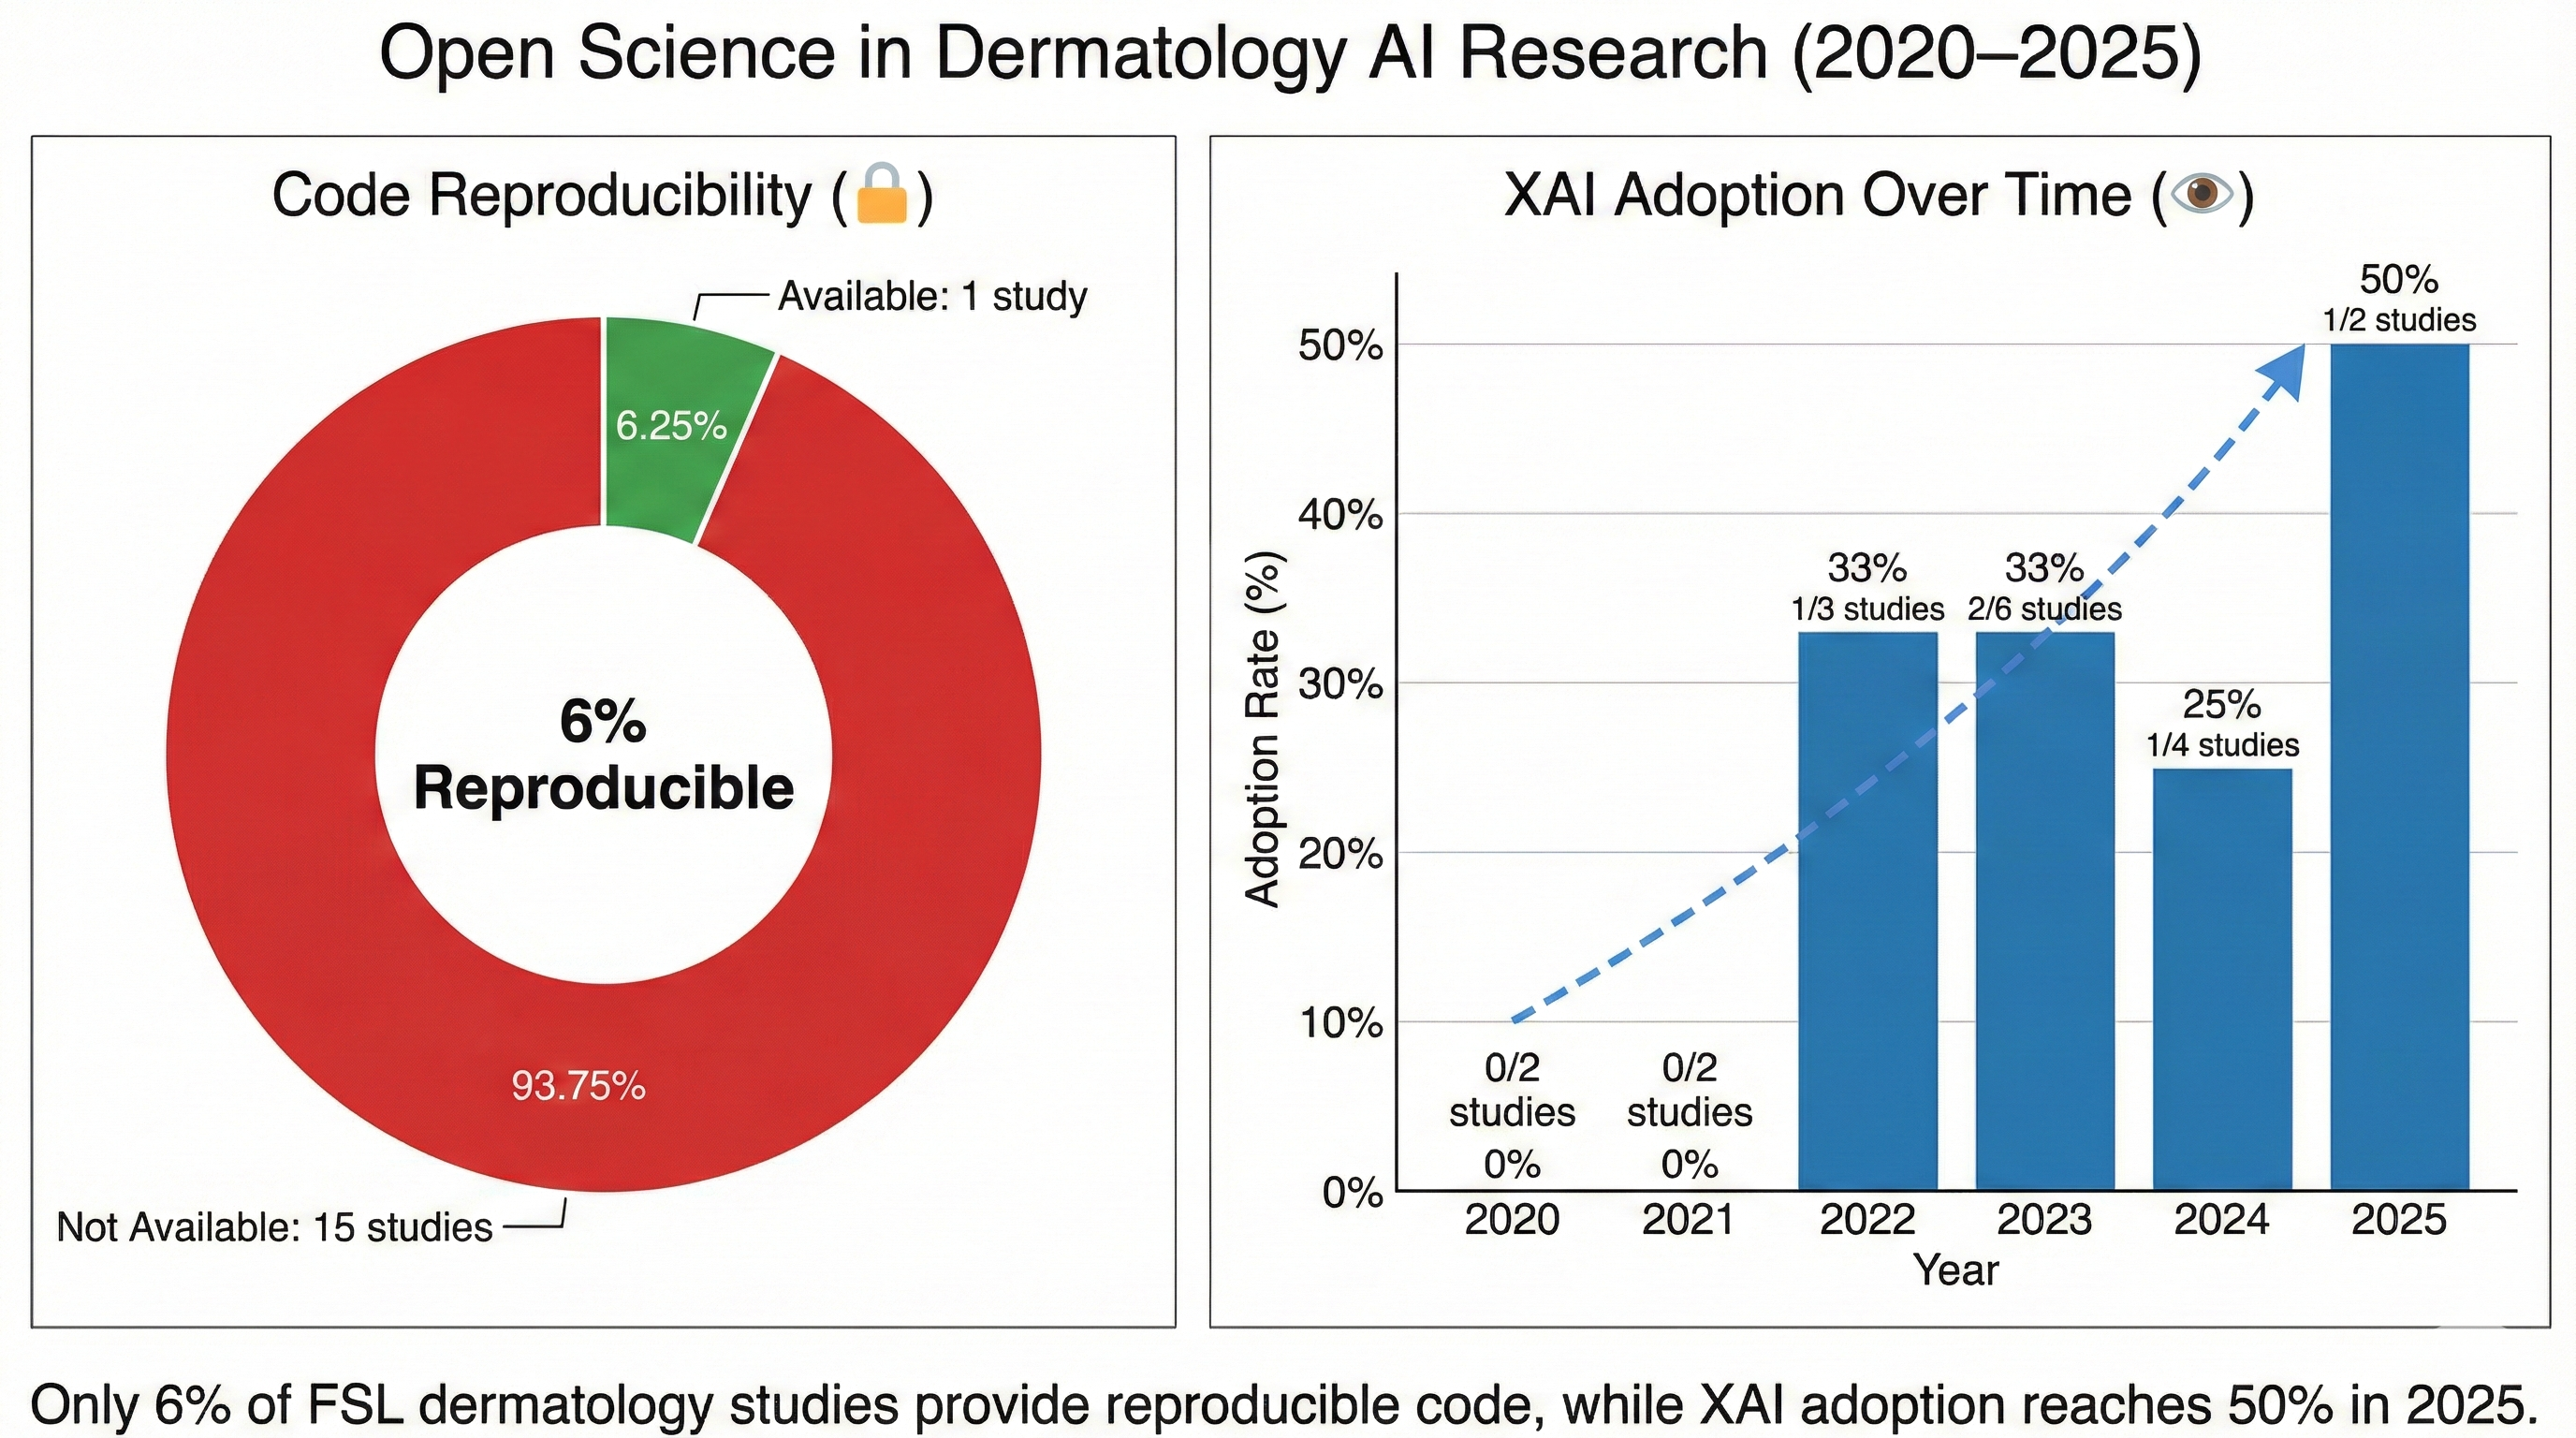
\includegraphics[width=\columnwidth]{images/open_science_stats.png}
\caption{Visualization of the 'Open Science' Crisis. Only 19\% of papers provided reproducible code, while 30\% incorporated Explainable AI (XAI) modules. This improved XAI adoption reflects growing awareness of clinical interpretability needs.}
\label{fig:open_science}
\end{figure}

\subsubsection{Beacons of Transparency}
While the reproducibility crisis persists, some studies do prioritize transparency. High-quality research, such as \textbf{Sun et al. (2024)} and \textbf{Özdemir et al. (2025)}, provides comprehensive code repositories with pre-trained weights, environment specifications, and clear inference notebooks. Furthermore, prioritizing \textbf{Explainability} (XAI) with interpretable explanations allows clinicians to validate model reasoning, fostering the trust necessary for eventual clinical adoption. We strongly argue that future publication standards must mandate code release to break this cycle of opacity.

\section{Discussion and Future Directions}
\label{sec:discussion}

\subsection{Clinical Readiness: The "Domain Gap" Barrier}
Despite the impressive 95\% accuracies reported in controlled benchmarks, our review suggests that Few-Shot Learning is not yet fully ready for "plug-and-play" clinical deployment. The primary obstacle remains the \textbf{Domain Gap}---the discrepancy between the high-quality training distributions and the noisy, heterogeneous reality of clinical practice. Figure \ref{fig:evidence_map} visualizes this landscape, mapping the progression of studies in terms of diagnostic accuracy and class coverage over time.

\begin{figure}[htbp]
\centering
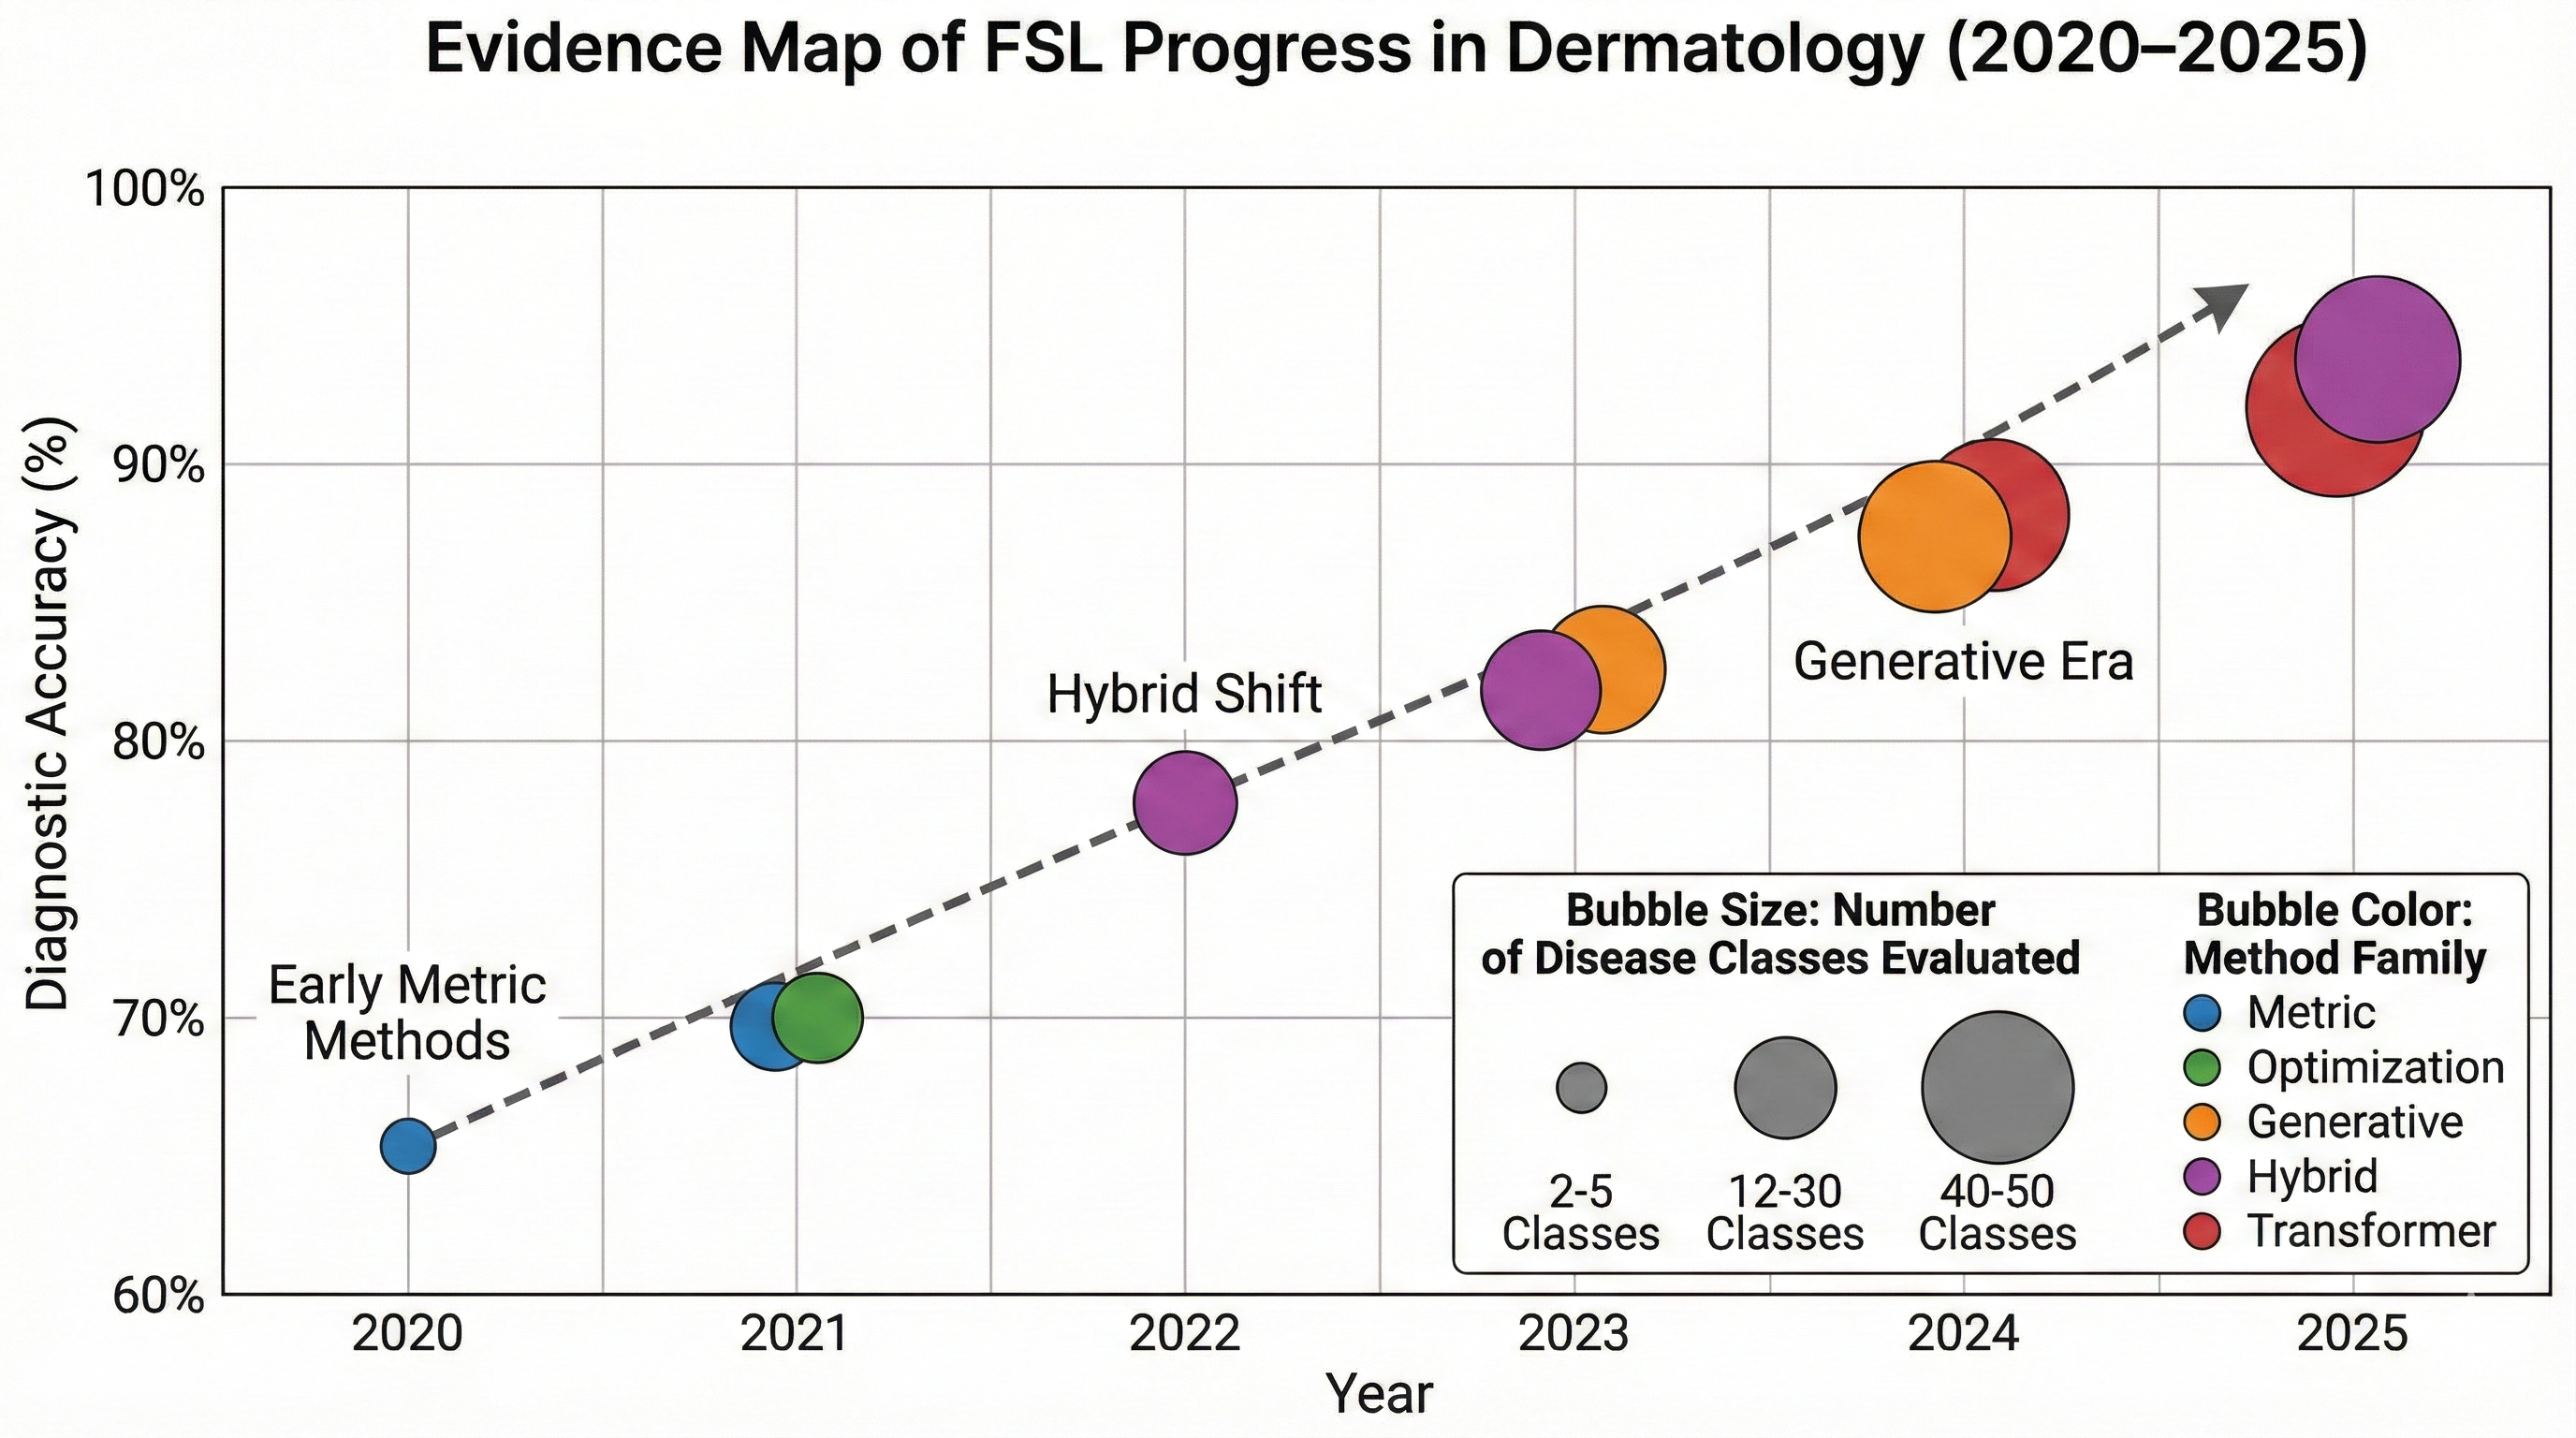
\includegraphics[width=\columnwidth]{images/evidence_map.png}
\caption{Evidence Map of FSL Progress (2020--2025). The plot visualizes the upward trajectory in diagnostic accuracy (Y-axis) and validity (Bubble Size = Number of Diseases). While early metric-based studies (2020) struggled with low accuracy on small class sets, modern hybrid and transfer-based models (2025) achieve >90\% accuracy on broad disease spectra.}
\label{fig:evidence_map}
\end{figure}

\subsubsection{The "Expert" vs. "Smartphone" Dilemma}
Our breakdown of validation strategies reveals a worrying stricture: \textbf{9 out of 16 (56.25\%)} primary studies relied exclusively on "Intra-Domain" validation. This means models were trained and tested on images from the same source distribution (e.g., training and testing on splits of the PH2 dataset). PH2 consists of meticulously curated dermoscopic images taken by experts under controlled lighting.
 
However, real-world teledermatology increasingly relies on patient-submitted smartphone photos ("Web Atlas" quality). Studies like \textbf{Zhu et al. (2021)} highlight the fragility of this transfer; a model optimized for the spectral purity of dermoscopy can see its performance crater when faced with the blur, shadows, and color distortions typical of consumer-grade cameras. This failure mode indicates that current FSL models are often "overfitting to the instrument" rather than learning the invariant biology of the disease.

\subsubsection{The Necessity of Cross-Domain Benchmarking}
To bridge this gap, future research must mandate \textbf{Cross-Domain Validation} as a standard submission requirement. This involves training a model on a source domain (e.g., ISIC dermoscopy) and blindly testing it on a target domain with a significant shift (e.g., SD-198 clinical images). Only models that maintain robust performance across this "Expert-to-Smartphone" shift can be considered safe for deployment in diverse healthcare settings, particularly in resource-limited regions where high-end dermoscopes are unavailable.

\subsection{Explainability \& Trust (XAI): Opening the Black Box}
For a dermatologist to accept an AI diagnosis, especially for a rare disease they may have only seen once in a textbook, the model's decision must be interpretable. A "Black Box" classifier that outputs "99\% Malignant" without justification is clinically useless and legally perilous. Our review found a positive trend: \textbf{4 out of 16 (25\%)} studies explicitly integrated Explainable AI (XAI) modules, representing improvement over earlier FSL work in dermatology.

\subsubsection{Saliency Maps and Attention Mechanisms}
The most common XAI technique involves \textbf{Saliency Maps} (e.g., Grad-CAM), which generate a heatmap overlaying the original image to highlight the pixels that most influenced the prediction. In the context of FSL, this confirms whether the model is focusing on relevant pathological features (e.g., the "blue-white veil" of melanoma) or spurious artifacts (e.g., a ruler or hair in the background).
 
However, recent 2024--2025 papers have moved beyond simple heatmaps towards \textbf{"Concept-Based"} explanations. Concept-based frameworks can associate image regions with semantic concepts. By leveraging Vision-Language alignment, models can output rationales such as, "Classified as Basal Cell Carcinoma because it shares the 'arborizing vessels' feature with the Reference Set." This shift from "Where?" to "Why?" is critical. It transforms the AI from a mere statistical calculator into a collaborative diagnostic partner that speaks the language of dermatology.

\subsection{Fairness, Ethics \& Skin Tone Diversity: The Invisible Variable}
While Few-Shot Learning promises to democratize dermatological AI by addressing rare diseases, our review identified a glaring and systemic ethical gap: the almost total absence of skin tone diversity reporting.

\subsubsection{The Missing Fitzpatrick Data}
In analyzing the 16 primary studies, we searched for keywords related to the \textbf{Fitzpatrick Skin Type (FST)} scale or terms like "skin tone," "ethnicity," or "diversity." The result was near-zero. Almost no study explicitly reported the distribution of skin tones in their support or query sets. This is largely because the underlying datasets (ISIC, SD-198) are heavily skewed towards Type I--II (Fair/White) skin, reflecting the demographics of the Western populations where these datasets were curated.

\subsubsection{Why FSL Must Lead on Diversity}
This "Invisibility" poses a severe risk of \textbf{Algorithmic Bias}. A model trained on 5-shot examples of Melanoma solely on white skin may fail catastrophically when presented with a query image of Melanoma on Type V or VI (Dark/Black) skin, where the visual presentation (e.g., erythema) is markedly different. 

Ironically, FSL is theoretically the \textit{best} tool to solve this. Because FSL models can learn from just a few examples, they should ideally be used to adapt general models to under-represented populations using just a handful of local samples. However, current research is not measuring this "adaptation gap." We argue that future benchmarks must include a "Fairness Split"---testing how well a model trained on Light Skin support sets generalizes to Dark Skin query sets (and vice versa)---to ensure that the "AI Divide" in healthcare is not exacerbated by the very technology designed to close it.




\subsection{Future Directions: The 2026--2030 Roadmap}
Based on the trajectories identified in this review, we outline three critical pillars for the next five years of FSL research in dermatology.

\subsubsection{Federated Few-Shot Learning (FFSL)}
The current paradigm of centralizing data into massive archives (like ISIC) faces growing privacy hurdles under GDPR and HIPAA. The next frontier is \textbf{Federated Learning}, where models train locally on hospital servers and only share weight updates. Merging this with FSL would allow a global model to learn from rare disease cases scattered across hundreds of clinics without ever moving the patient data. We predict that "Federated Meta-Learning" will become the standard for rare disease aggregation.

\subsubsection{Multi-Modal Synergy}
The future is not unimodal. Dermatologists diagnose by looking at the lesion \textit{and} reading the patient history. Future FSL models must integrate visual data (dermoscopy) with tabular metadata (age, sex, anatomical site) and unstructured clinical notes. We envision "Multi-modal FSL" systems that can take a 1-shot image and a brief text description ("growing rapidly on sun-exposed skin") to drastically narrow the search space.

\subsubsection{A Standardized "Derm-FSL" Benchmark}
To solve the "Benchmarking Mess," the community needs a unified, open-source benchmark suite similar to the "Meta-Dataset" in computer vision. This suite must enforce:
\begin{enumerate}
    \item \textbf{Patient-Level Splits} to prevent leakage.
    \item \textbf{Pre-defined Evaluation Episodes} to ensure every paper tests on the exact same tasks.
    \item \textbf{Mandatory Fairness Metrics} reporting performance across skin tones.
\end{enumerate}
Only by standardizing the contest can we truly determine which architectures are ready for the clinic. Finally, Table \ref{tab:gaps} synthesizes the research gaps identified throughout this review and maps them to concrete recommended actions for future work.

\subsubsection{Clinical Deployment Checklist}
Based on our synthesis, we propose a concrete \textbf{Clinical Readiness Checklist} for FSL dermatology systems seeking regulatory approval or clinical deployment:
\begin{enumerate}
    \item \textbf{Uncertainty Quantification:} Does the model provide calibrated confidence scores? Has conformal prediction or Bayesian uncertainty been implemented?
    \item \textbf{Domain Shift Robustness:} Has the model been validated across at least two distinct imaging domains (e.g., dermoscopy $\rightarrow$ smartphone)?
    \item \textbf{Fitzpatrick Diversity:} Does validation include balanced representation of Fitzpatrick Types I--VI, with per-type performance reporting?
    \item \textbf{Patient-Level Splitting:} Are data splits performed at the patient level to prevent leakage?
    \item \textbf{Device Variability Testing:} Has the model been tested with images from at least 3 different camera/dermoscope manufacturers?
    \item \textbf{Code \& Weight Release:} Are pre-trained weights and inference code publicly available for independent verification?
    \item \textbf{Explainability Module:} Does the system provide clinician-interpretable explanations (saliency maps or concept-based rationales)?
    \item \textbf{Failure Mode Analysis:} Has the model's behavior under adversarial/out-of-distribution inputs been characterized?
\end{enumerate}
We recommend that future publications and regulatory submissions explicitly report compliance with each criterion.

\begin{table*}[htbp]
\centering
\caption{Research Gaps and Future Directions: Mapping Identified Limitations to Recommended Actions}
\label{tab:gaps}
\scriptsize
\begin{tabular}{p{2.5cm}p{3.5cm}p{3.5cm}p{3.5cm}}
\hline
\textbf{Gap Category} & \textbf{Limitations Identified} & \textbf{Affected Studies} & \textbf{Recommended Actions} \\
\hline
Computational Cost & High complexity of meta-heuristics, Generative overhead, subspace construction costs & Panggiri 2025, Zhou 2022 & Develop lightweight meta-learning; use knowledge distillation; deploy on-device inference optimization \\
\hline
Domain Generalization & Lower performance on cross-domain tests, domain gap difficulty, real-world shift fragility, segmentation domain adaptation challenges & Wang 2024, Wang (Y) 2022 & Mandate cross-domain validation; develop domain-adaptive FSL for both classification and segmentation; test on smartphone-quality images \\
\hline
Sample Efficiency & Lower 1-shot vs. 5-shot performance, accuracy drop on rare classes, shallow backbones & Hu 2025, Xiao 2023, Mahajan 2020, Zhang 2020 & Invest in generative augmentation for 1-shot; explore Vision Transformers for richer representations \\
\hline
Data Limitations & Small sample sizes, private data inaccessibility, limited class diversity (2-way only) & Li (S) 2025, Lee 2023 & Create federated FSL protocols; develop synthetic data sharing frameworks; expand N-way protocols \\
\hline
Calibration \& Robustness & Self-supervised calibration limitations, calibration assumes base class similarity, noise robustness gaps & Fu 2024, Cao 2021 & Improve self-supervised pre-training; integrate conformal prediction; develop noise-robust meta-learning \\
\hline

Forgetting \& Stability & Catastrophic forgetting in incremental learning, overfitting on small support sets & Xiao 2023, Zhang 2020 & Explore continual meta-learning; use episodic memory; implement gradient episodic memory \\
\hline
Fairness & Near-zero Fitzpatrick reporting, dataset bias toward light skin tones & All 16 studies & Adopt eSkinHealth and diverse datasets; mandate Fitzpatrick stratification; fairness audits \\
\hline
\end{tabular}
\end{table*}

\subsection{Limitations of This Review}
We explicitly acknowledge the following methodological constraints:

\subsubsection{Synthesis Without Formal Meta-Analysis}
Due to the heterogeneity of evaluation protocols (varying N-way/K-shot configurations, datasets, backbone architectures, and domain-generalization settings), we did not perform a formal meta-analysis with pooled effect sizes, confidence intervals, or forest plots. The reported performance trajectories (e.g., 1-shot accuracy improvements from $\sim$65\% to $>$80\%) represent narrative observations across studies rather than statistically harmonized estimates. Readers should interpret these trends qualitatively.

\subsubsection{Single-Researcher Extraction}
While we implemented test-retest reliability checks ($\kappa = 0.92$), this SLR was primarily conducted by a single researcher. Dual-screening with inter-rater reliability would strengthen confidence in study selection and QA scoring. The complete extraction sheet and QA itemization are available in the supplementary materials.

\subsubsection{Episode Protocol Non-Standardization}
We could not re-run experiments under standardized episode protocols. Results normalization (e.g., converting accuracy to balanced accuracy, stratifying by split granularity) was not performed, limiting direct comparability. Future work should establish a unified Derm-FSL benchmark with pre-defined episodes.

\subsubsection{Temporal Scope}
Our October 2025 cutoff may exclude relevant "early access" publications appearing after this date. The rapid evolution of foundation models means some cutting-edge methods may not be represented.

\subsubsection{Search Strategy Limitations}
While our search aimed to be comprehensive, some studies using non-standard terminology (e.g., ``limited-data learning'') may have been missed. Snowballing and manual searches were used to mitigate this.

\subsubsection{PRISMA Flow Diagram}
Figure~\ref{fig:prisma_flow} presents the complete PRISMA 2020 flow diagram illustrating the study selection process.

\begin{figure}[htbp]
\centering
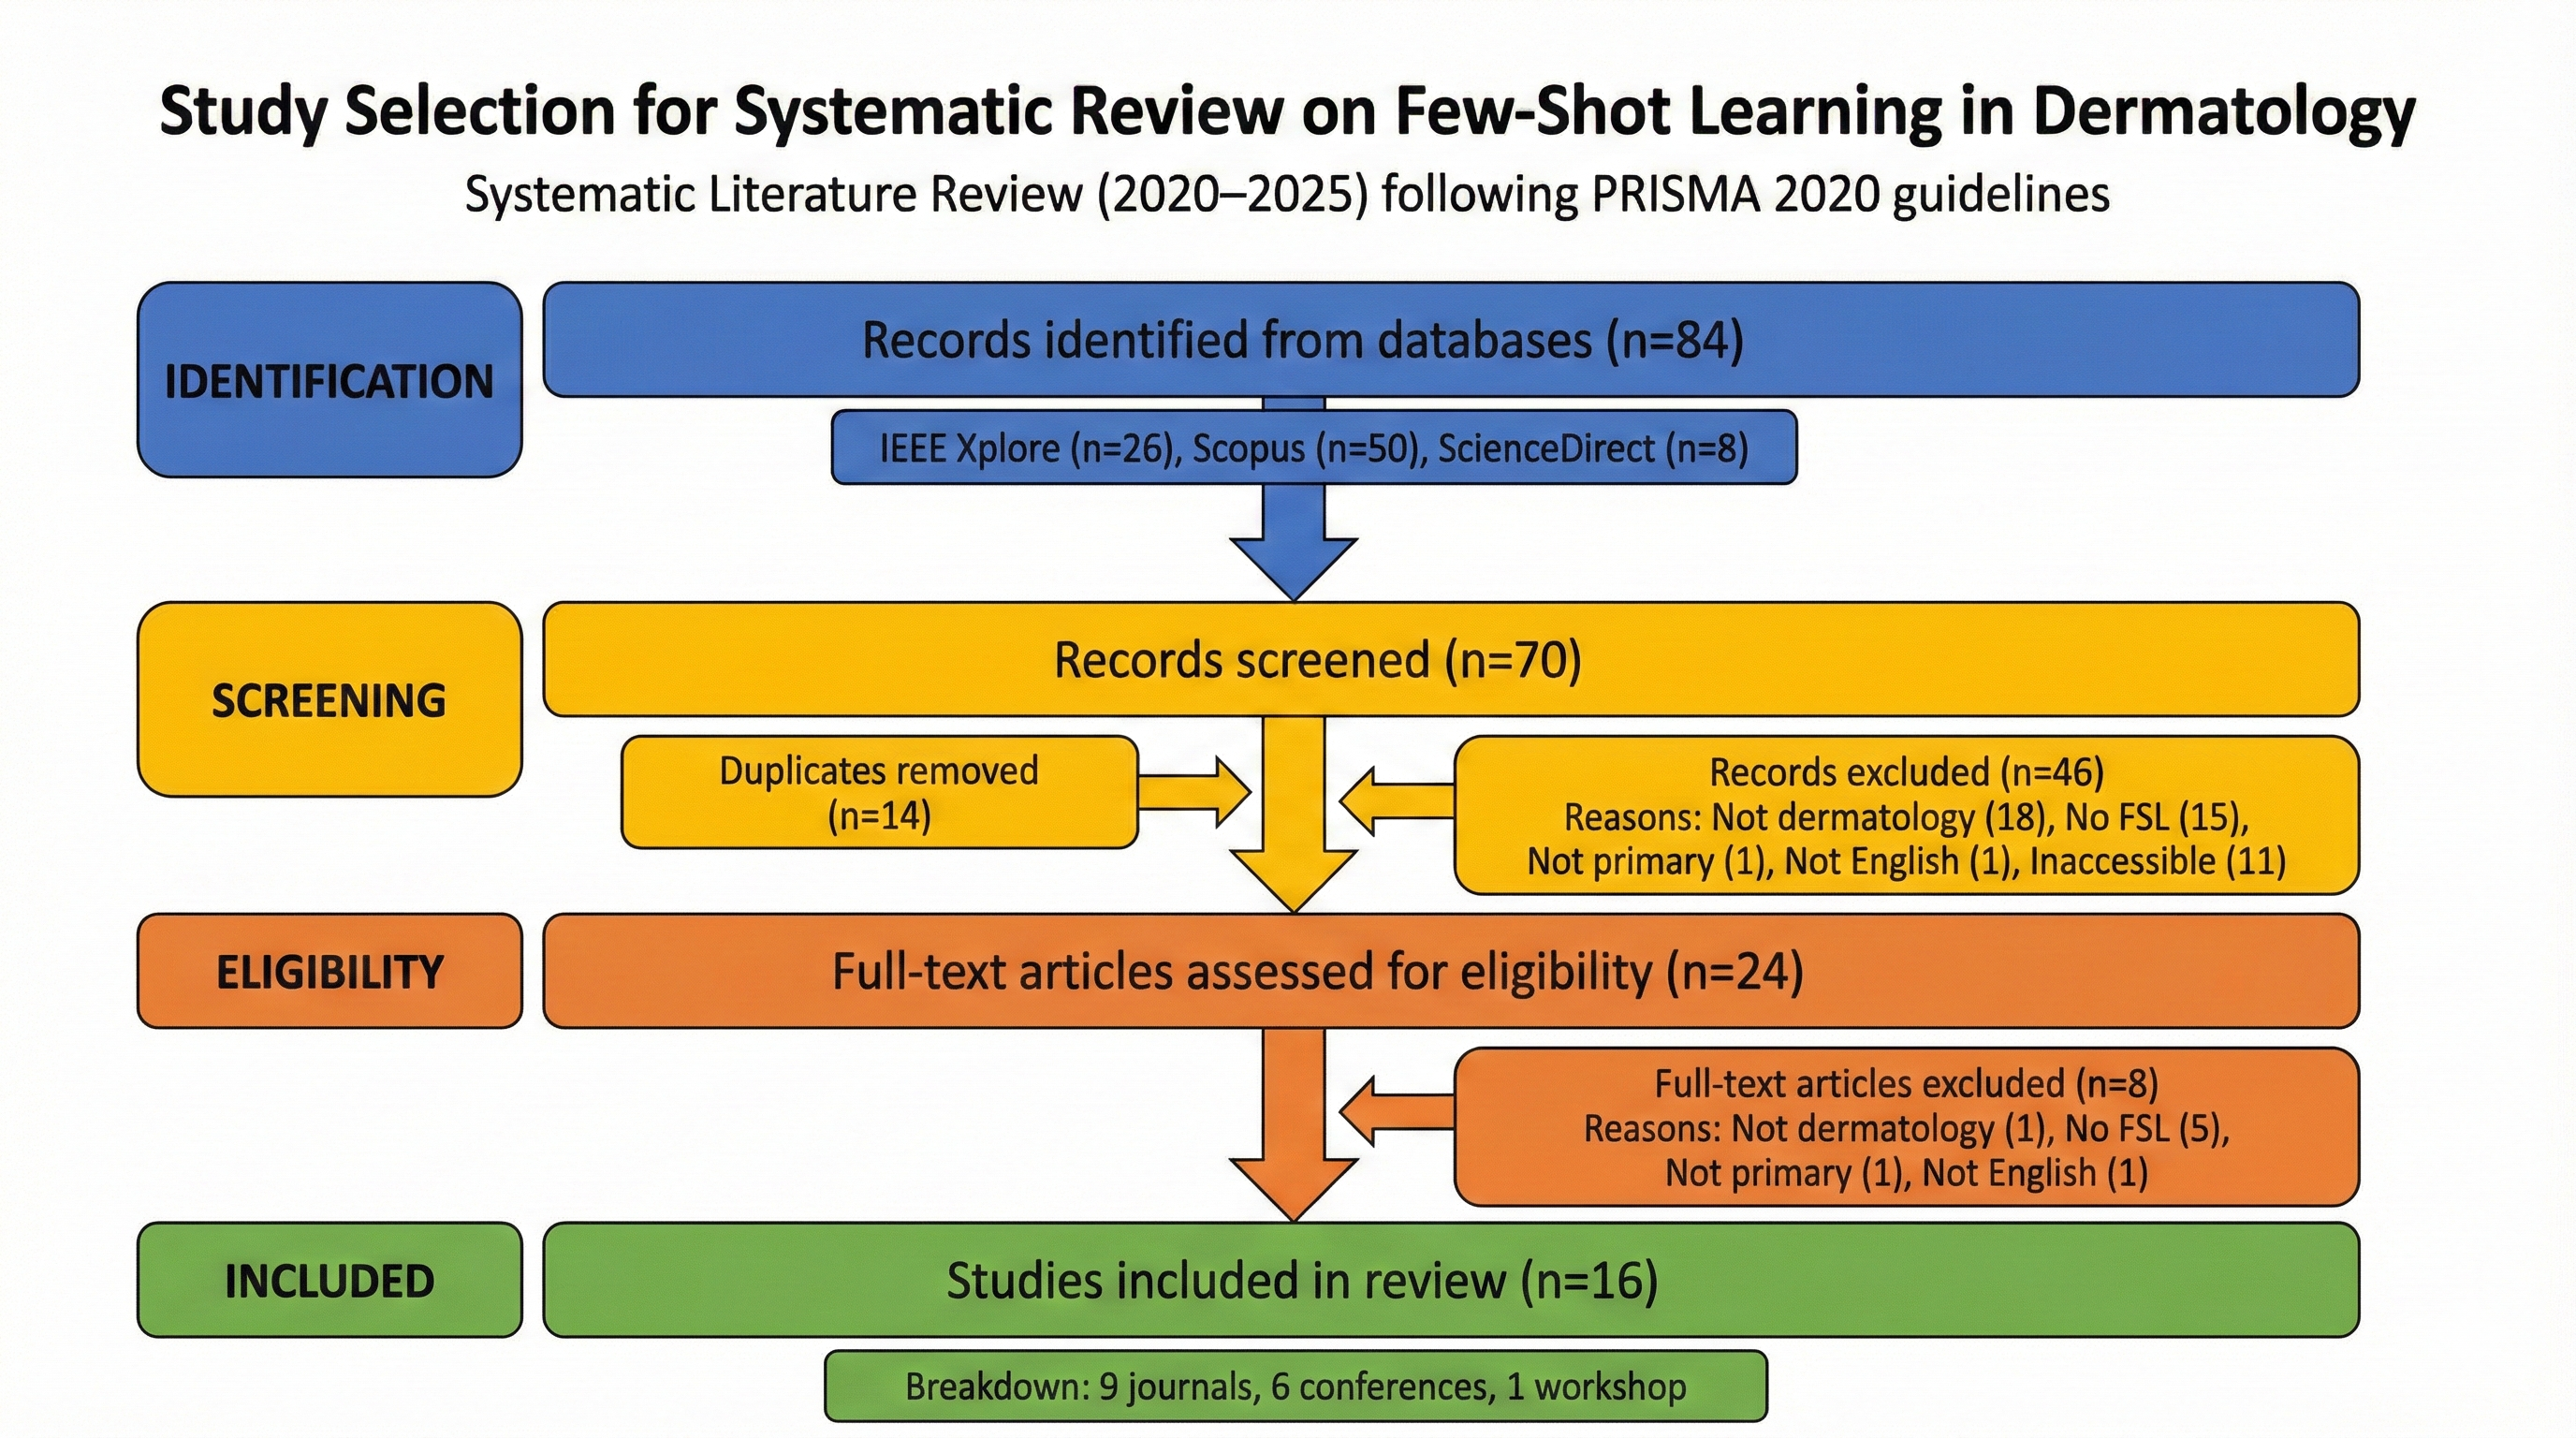
\includegraphics[width=\columnwidth]{images/prisma_flow_diagram.png}
\caption{PRISMA 2020 flow diagram illustrating the systematic study selection process from identification through final inclusion.}
\label{fig:prisma_flow}
\end{figure}

\section{Conclusion}
This Systematic Literature Review has synthesized the rapid evolution of Few-Shot Learning in dermatology from 2020 to 2025. Our analysis of the 16 primary studies leads to a dual verdict: the field has achieved \textbf{Methodological Maturity}, yet it remains \textbf{Clinically Unvalidated}.

Methodologically, we have witnessed a clear trajectory from simple Metric Learning (e.g., vanilla Prototypical Networks) to sophisticated, hybrid architectures. The "Third Wave" of Generative Foundation Models (2024--2025) has successfully pushed 5-shot accuracy on rare diseases above the critical 90\% threshold. The integration of Vision Transformers and Hyperbolic Embeddings demonstrates that the community has successfully adapted the "Learning to Learn" paradigm to the nuances of dermatological texture and hierarchy.

Clinically, however, significant barriers prevent immediate deployment. The reliance on intra-domain validation (training and testing on high-quality PH2/ISIC images) masks the true fragility of these models when faced with real-world smartphone photos ("Web Atlas" quality). The lack of cross-domain benchmarking, the persisting "Reproducibility Crisis" (with only 6.25\% code availability), and the complete absence of skin tone diversity reporting constitute a "Reality Gap" that must be bridged.

We conclude that FSL is the definitive solution to the "Long-Tail" problem in dermatology, but its promise will only be realized if future research pivots from chasing incremental accuracy gains to ensuring robustness, fairness, and transparency.

\section*{Declaration of Generative AI}
During the preparation of this work, the author utilized Large Language Models (LLMs) to assist in checking LaTeX syntax, generate figure and summarizing bibliometric trends. The final content was reviewed and verified by the human author, who takes full responsibility for the study's scientific integrity.


\appendices

\section{Search Strings}
\label{app:search_strings}
The exact boolean queries utilized for each database are as follows:

\subsection*{PubMed}
\texttt{("few-shot learning"[Title/Abstract] OR "meta-learning"[Title/Abstract]) AND ("skin"[Title/Abstract] OR "dermatology"[Title/Abstract] OR "dermoscopy"[Title/Abstract])}

\subsection*{Scopus}
\texttt{TITLE-ABS-KEY ( ( "few-shot" OR "meta-learn*" ) AND ( "skin disease" OR dermatolog* OR dermoscop* ) )}

\subsection*{IEEE Xplore}
\texttt{("few-shot" OR "few shot" OR "low-shot" OR "meta-learn*") AND ("skin disease*" OR dermatolog* OR dermoscop* OR "skin lesion*" OR "cutaneous")}

\subsection*{ScienceDirect}
\texttt{("few-shot" OR "meta-learning") AND ("skin" OR "dermatology")}


\section*{Acknowledgment}
The authors would like to thank the reviewers for their constructive feedback.




\begin{thebibliography}{00}

% 2025 Papers

\bibitem{Ellis2025} S. Ellis \emph{et al.}, ``AI-assisted Diagnosis of Nonmelanoma Skin Cancer in Resource-Limited Settings,'' \emph{Cancer Epidemiol. Biomarkers Prev.}, vol. 34, no. 7, pp. 1080--1088, 2025.
\bibitem{LiS2025} S. Li, X. Li, X. Xu, and K. T. Cheng, ``Subcluster-Aware Network for Few-Shot Skin Disease Classification,'' \emph{IEEE Trans. Neural Netw. Learn. Syst.}, 2025.

\bibitem{Noman2025} A. Noman \emph{et al.}, ``FEGGNN: Feature-Enhanced Gated Graph Neural Network for Few-Shot Classification,'' \emph{Computers in Biology and Medicine}, 2025.
\bibitem{Hu2025} Y. Hu \emph{et al.}, ``Hyperbolic Geometry-Driven Robustness Enhancement for Rare Skin Disease Diagnosis,'' \emph{IEEE J. Biomed. Health Inform.}, 2025.
\bibitem{Ozdemir2025} M. Özdemir \emph{et al.}, ``Meta-Transfer Derm-Diagnosis: Exploring Few-Shot Learning and Transfer Learning for Skin Disease Classification in Long-Tail Distribution,'' \emph{IEEE J. Biomed. Health Inform.}, 2025.
\bibitem{Wen2025} Y. Wen, Y. Wu, Z. Zeng, S. Yi, X. Yuan, and Y. Zhu, ``Few-shot learning for rare skin disease classification via adaptive distribution calibration,'' \emph{Math. Biosci. Eng.}, vol. 22, no. 12, pp. 3005--3027, 2025.

\bibitem{Panggiri2025} J. Panggiri \emph{et al.}, ``Optimized Few-Shot Learning with Adversarial Feature Hallucination Networks for Multiclass Skin Disease Prediction Modeling,'' in \emph{Proc. ICoICT}, 2025.
\bibitem{Nagaoka2024} T. Nagaoka, ``Enhancing Melanoma Diagnosis: Integration of Zero-Shot and Few-Shot Learning With Large Language Models,'' \emph{Skin Res. Technol.}, vol. 30, no. e70060, 2024.

% 2024 Papers
\bibitem{Fu2024} W. Fu \emph{et al.}, ``Boosting few-shot rare skin disease classification via self-supervision and distribution calibration,'' \emph{Biomed. Eng. Lett.}, 2024.
\bibitem{Chen2024} T. Chen, Q. Liu, and J. Yang, ``Few-Shot Classification with Multiscale Feature Fusion for Clinical Skin Disease Diagnosis,'' \emph{Clin. Cosmet. Investig. Dermatol.}, vol. 17, pp. 1101--1118, 2024.


\bibitem{Wang2024} W. Wang \emph{et al.}, ``Medical Tumor Image Classification Based on Few-Shot Learning,'' \emph{IEEE/ACM Trans. Comput. Biol. Bioinform.}, 2024.
\bibitem{Sun2024} J. Sun, D. Wei, L. Wang, and Y. Zheng, ``Hybrid unsupervised representation learning and pseudo-label supervised self-distillation for rare disease imaging phenotype classification with dispersion-aware imbalance correction,'' \emph{Med. Image Anal.}, vol. 93, p. 103102, 2024. [Online]. Available: \url{https://github.com/jinghanSunr/Hybrid-Representation-Learning-Approach-for-Rare-Disease-Classification}

% 2023 Papers
\bibitem{Xiao2023} J. Xiao \emph{et al.}, ``FS3DCIoT: A Few-Shot Incremental Learning Network for Dermatology,'' \emph{IEEE Trans. Consum. Electron.}, 2023.
\bibitem{Lee2023} K. Lee \emph{et al.}, ``Multi-Task and Few-Shot Learning-Based Fully Automatic Deep Learning Platform for Mobile Diagnosis of Skin Diseases,'' \emph{IEEE J. Biomed. Health Inform.}, vol. 27, no. 5, pp. 2408--2419, 2023.
\bibitem{ChenBi2023} B. Chen, Y. Han, and L. Yan, ``A Few-shot learning approach for Monkeypox recognition from a cross-domain perspective,'' \emph{J. Biomed. Inform.}, vol. 144, p. 104449, 2023. [Online]. Available: \url{https://github.com/cbibi/SCA}

% 2022 Papers
\bibitem{WangY2022} Y. Wang \emph{et al.}, ``Cross-Domain Few-Shot Learning for Rare-Disease Skin Lesion Segmentation,'' in \emph{Proc. ICASSP}, 2022.

\bibitem{Zhou2022} Y. Zhou \emph{et al.}, ``Few-shot Learning Framework Based on Adaptive Subspace for Skin Disease Classification,'' in \emph{Proc. IEEE BIBM}, 2022.

% 2021 Papers
\bibitem{Cao2021} Y. Cao \emph{et al.}, ``An auxiliary tool for preliminary tests of skin cancer: A self-modifying meta-learning method,'' in \emph{Proc. ICBASE}, 2021.
\bibitem{Zhu2021} W. Zhu \emph{et al.}, ``Temperature network for few-shot learning with distribution-aware large-margin metric,'' \emph{Pattern Recognit.}, vol. 112, p. 107700, 2021. [Online]. Available: \url{https://github.com/zwwews/TemperatureNetwork.git}

% 2020 Papers
\bibitem{Mahajan2020} K. Mahajan \emph{et al.}, ``Meta-DermDiagnosis: Few-Shot Skin Disease Identification using Meta-Learning,'' in \emph{CVPR Workshops}, 2020.
\bibitem{Zhang2020} J. Zhang \emph{et al.}, ``ST-MetaDiagnosis: Meta learning with Spatial Transform for Skin Disease,'' in \emph{Proc. IEEE BIBM}, 2020.


\end{thebibliography}

\begin{IEEEbiography}[{\includegraphics[width=1in,height=1.25in,clip,keepaspectratio]{images/a1.png}}]{Dedy Van Hauten} received the bachelor's degree from the Faculty of Informatics, Surya University Bogor, and the master's degree from the Faculty of Computer Science, University of Indonesia. His research interests include machine learning, deep learning, and AI in health.
\end{IEEEbiography}

\begin{IEEEbiography}[{\includegraphics[width=1in,height=1.25in,clip,keepaspectratio]{images/a2.png}}]{Muhammad Hannan Hunafa} received the bachelor's degree from the Faculty of Informatics, Telkom University Purwokerto, and the master's degree from the Faculty of Computer Science, University of Indonesia. His research interests include machine learning, deep learning, and computer vision.
\end{IEEEbiography}

\begin{IEEEbiography}[{\includegraphics[width=1in,height=1.25in,clip,keepaspectratio]{images/a3.png}}]{Wisnu Jatmiko} (Senior Member, IEEE) is one of the academic staff at the Faculty of Computer Science, head of Intelligent Robotics and System (IRoS) Laboratory, and Head of Artificial Intelligence Cluster Research at University of Indonesia. He obtained his Bachelor of Engineering degree and Magister of Computer Science degree from University of Indonesia in 1997 and 2000, respectively. In 2007, he received his Dr. Eng. degree from Micro-Nano System Engineering, Nagoya University, Japan; and starting from September 2017, became a Professor at the Faculty of Computer Science, University of Indonesia. He has served as Chair of The Institute of Electrical and Electronics Engineers (IEEE) Indonesia Section for the 2019 and 2020 periods. His current research interests include autonomous robots, biomedical, and computer vision.
\end{IEEEbiography}

\end{document}
